\documentclass[../document.tex]{subfiles}
\begin{document}\label{ssec:time}
	
We first present execution time measurements for each benchmark, starting with the Cyclic Redundancy Check {\tt crc} benchmark which represents the Combinational Logic dwarf.

\newcommand{\plotwidth}{0.24\textwidth}
\begin{figure*}[t]
	\centering
	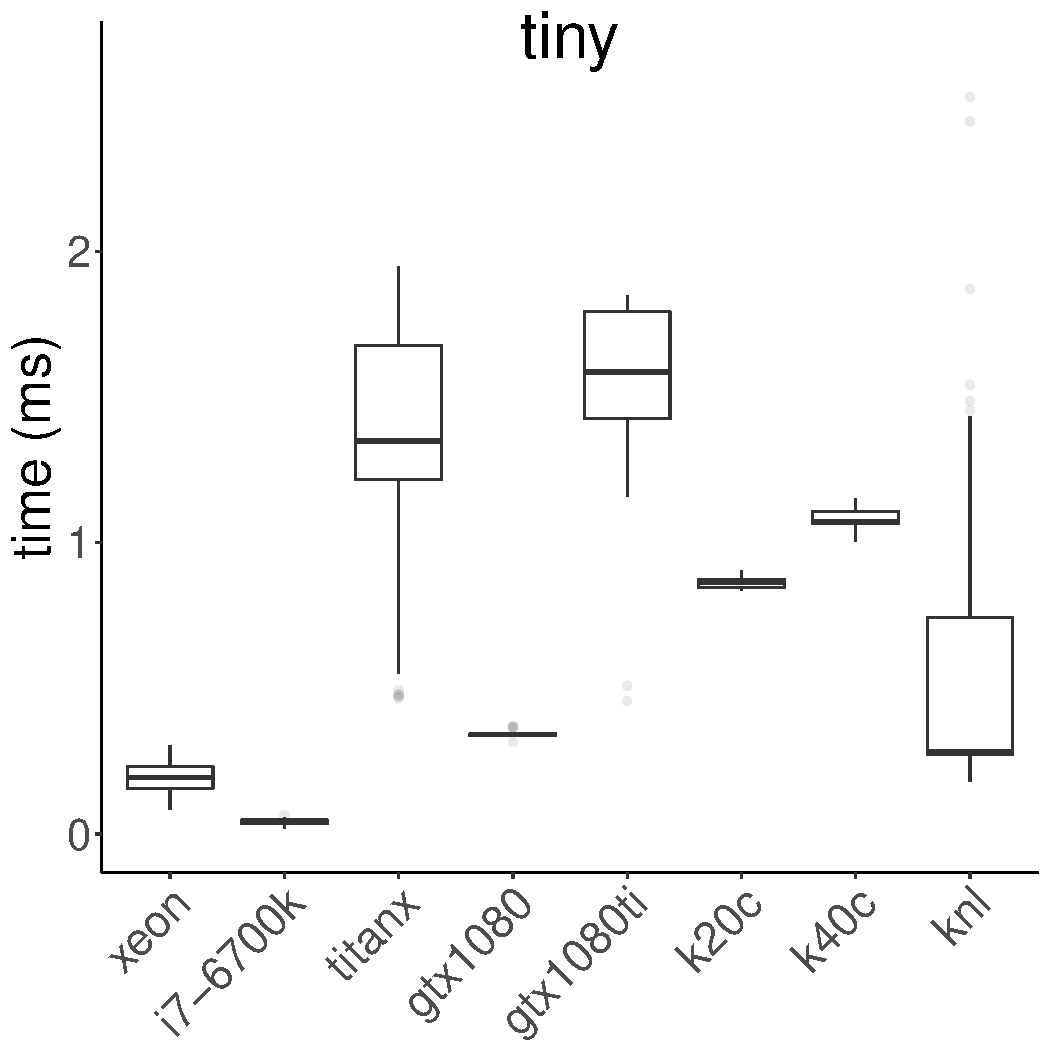
\includegraphics[width=\plotwidth]{figures/time-results/generate_crc_tiny_boxplot_knl-1}
	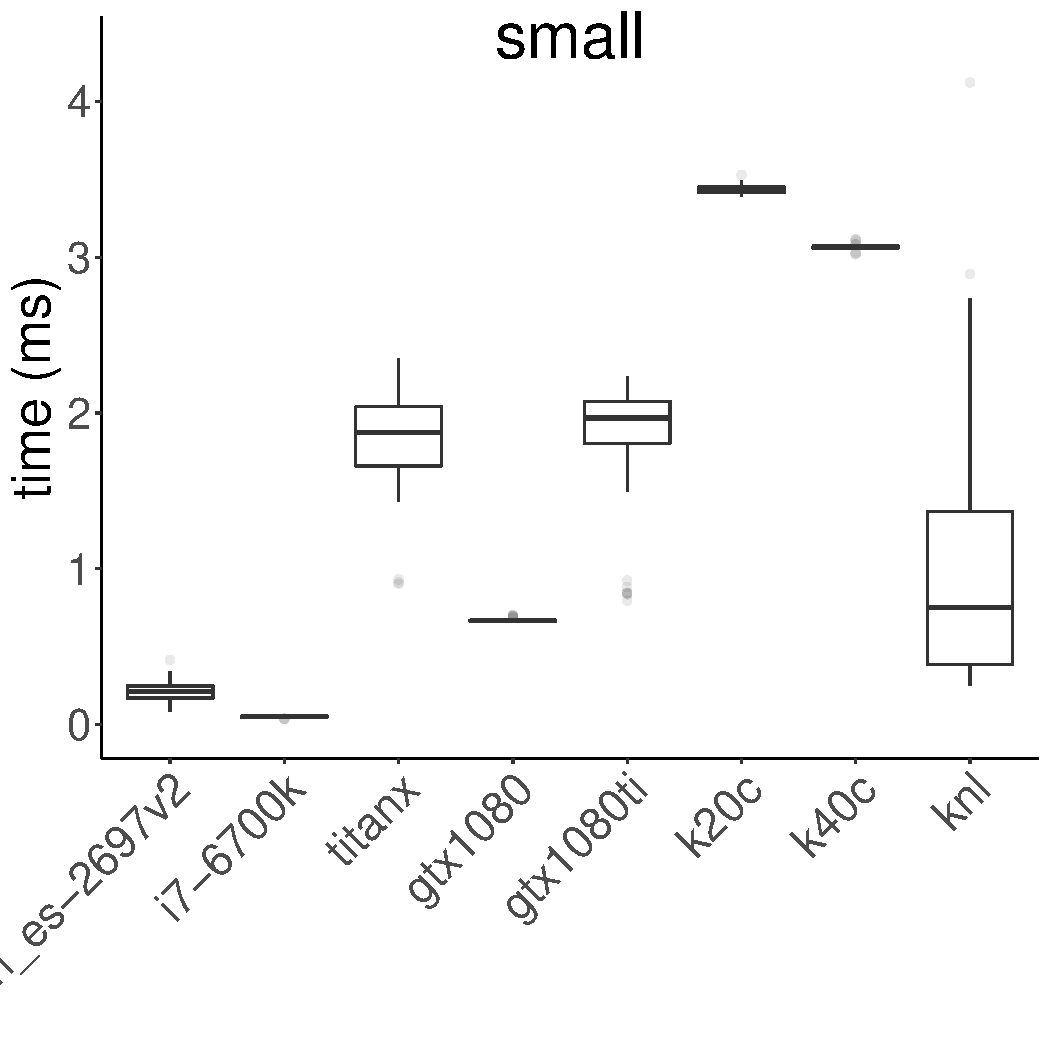
\includegraphics[width=\plotwidth]{figures/time-results/generate_crc_small_boxplot_knl-1}
	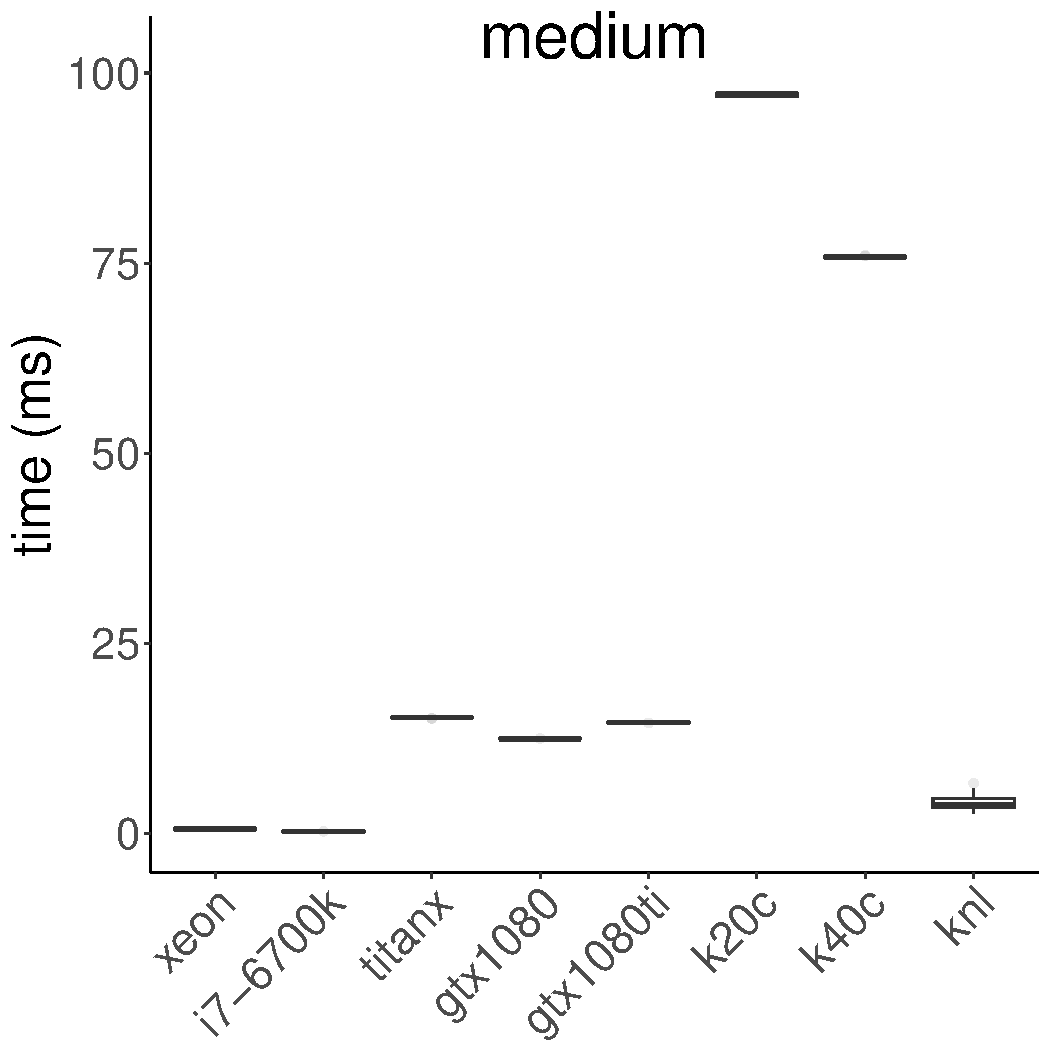
\includegraphics[width=\plotwidth]{figures/time-results/generate_crc_medium_boxplot_knl-1}
	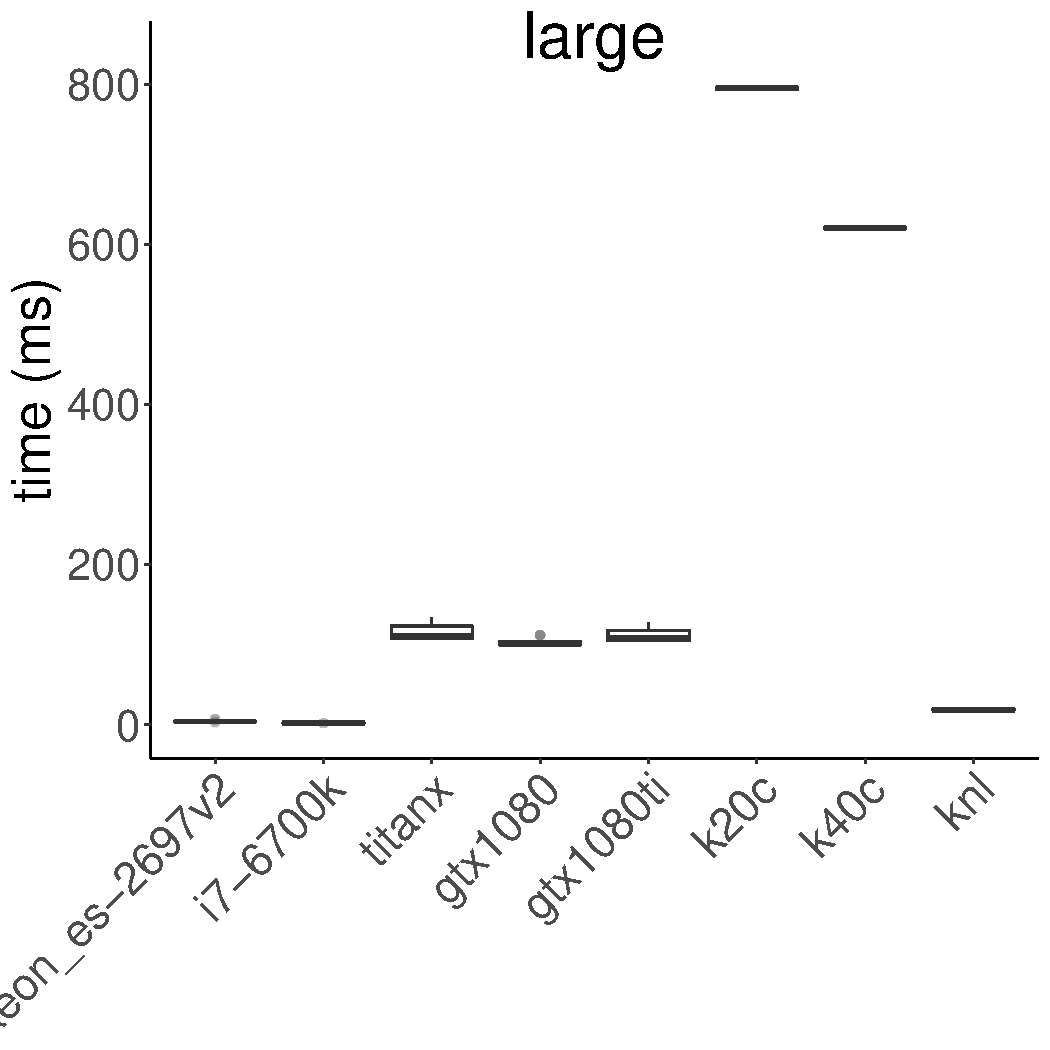
\includegraphics[width=\plotwidth]{figures/time-results/generate_crc_large_boxplot_knl-1}
	\caption{Kernel execution times for the {\bf crc} benchmark on different hardware platforms, including KNL}
	\label{fig:time-crc}
\end{figure*}

Figure~\ref{fig:time-crc} shows the execution times for the {\tt crc} benchmark over 50 iterations on each of the target architectures, including the KNL.
Execution times are lowest on CPU-type architectures, probably due to the low floating-point intensity of the CRC computation~\cite[Ch. 6]{joshi2016thesis}.
Excluding {\tt crc}, all the other benchmarks perform best on GPU type accelerators; furthermore, the performance on the KNL is poor due to the lack of support for wide vector registers in Intel's OpenCL SDK.
We therefore omit results for KNL for the remaining benchmarks.

\todo{We could examine the kiviat diagrams to see if they have high memory address entropy -- or high memory overhead which contributes to the why some benchmarks see a wide variation while others experience only a little, is this the major cause in variation?}
\todo{What are the major motivations for including this results section? We should conclude with these motivations and what has been shown accordingly}

Figures~\ref{fig:time} and~\ref{fig:time2} shows the distribution of kernel execution times for the remaining benchmarks.
Each benchmark corresponds to a particular dwarf: 
Figure~\ref{fig:time-kmeans} ({\tt kmeans}) represents the MapReduce dwarf,
Figure~\ref{fig:time-lud} ({\tt lud}) represents the Dense Linear Algebra dwarf,
Figure~\ref{fig:time-csr} ({\tt csr}) represents Sparse Linear Algebra, 
Figure~\ref{fig:time-dwt} ({\tt dwt}) and Figure~\ref{fig:time-fft} ({\tt fft}) represent Spectral Methods,
Figure~\ref{fig:time-gem} ({\tt gem}) represents N-Body Methods, 
and Figure~\ref{fig:time-srad} ({\tt srad}) represents the Structured Grid dwarf.

\captionsetup[subfigure]{justification=raggedright,singlelinecheck=false}

\begin{figure*}
	\begin{subfigure}{0.09\textwidth}\subcaption[l]{\bf kmeans} \label{fig:time-kmeans} \vspace{5mm}\end{subfigure}
	\begin{subfigure}{0.9\textwidth}
		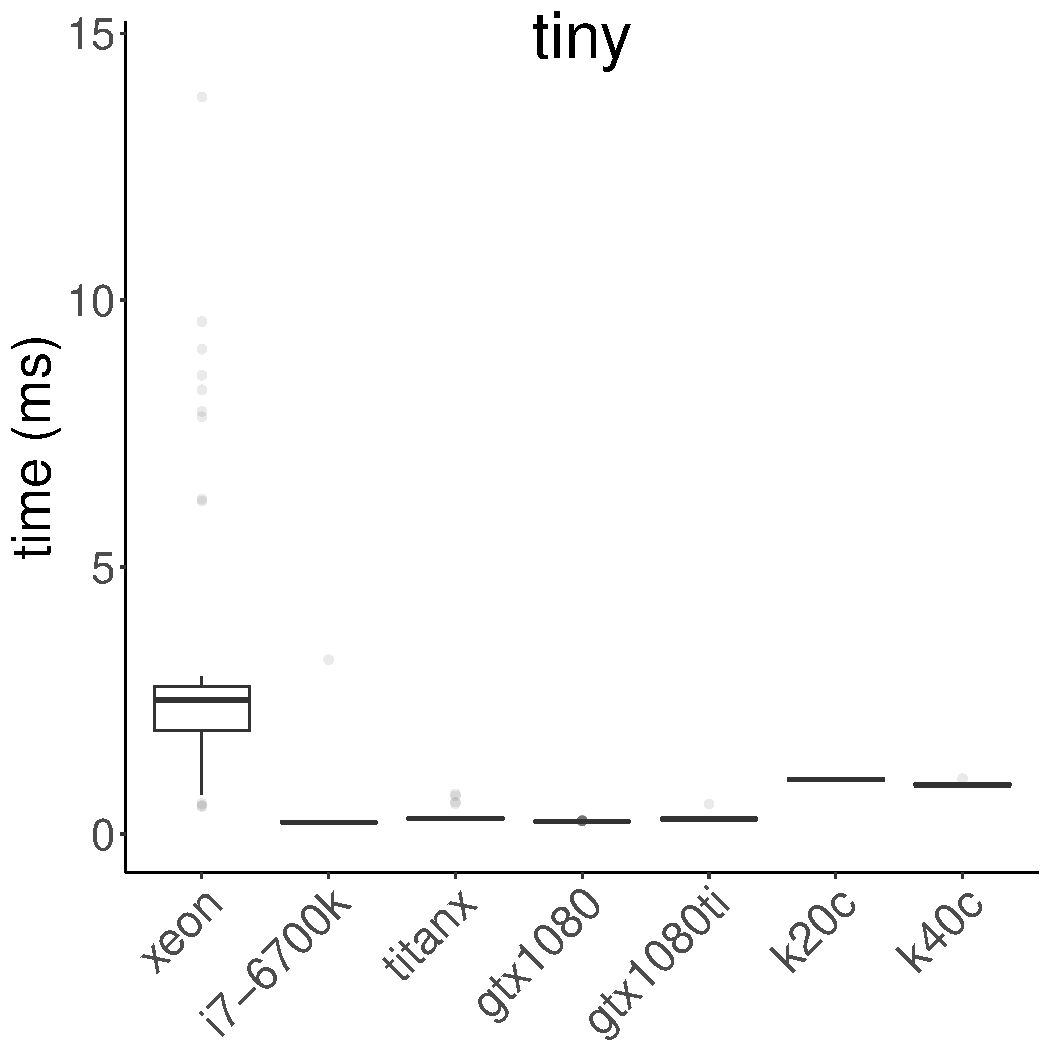
\includegraphics[width=\plotwidth]{figures/time-results/generate_kmeans_no_knl_tiny_boxplot-1}
		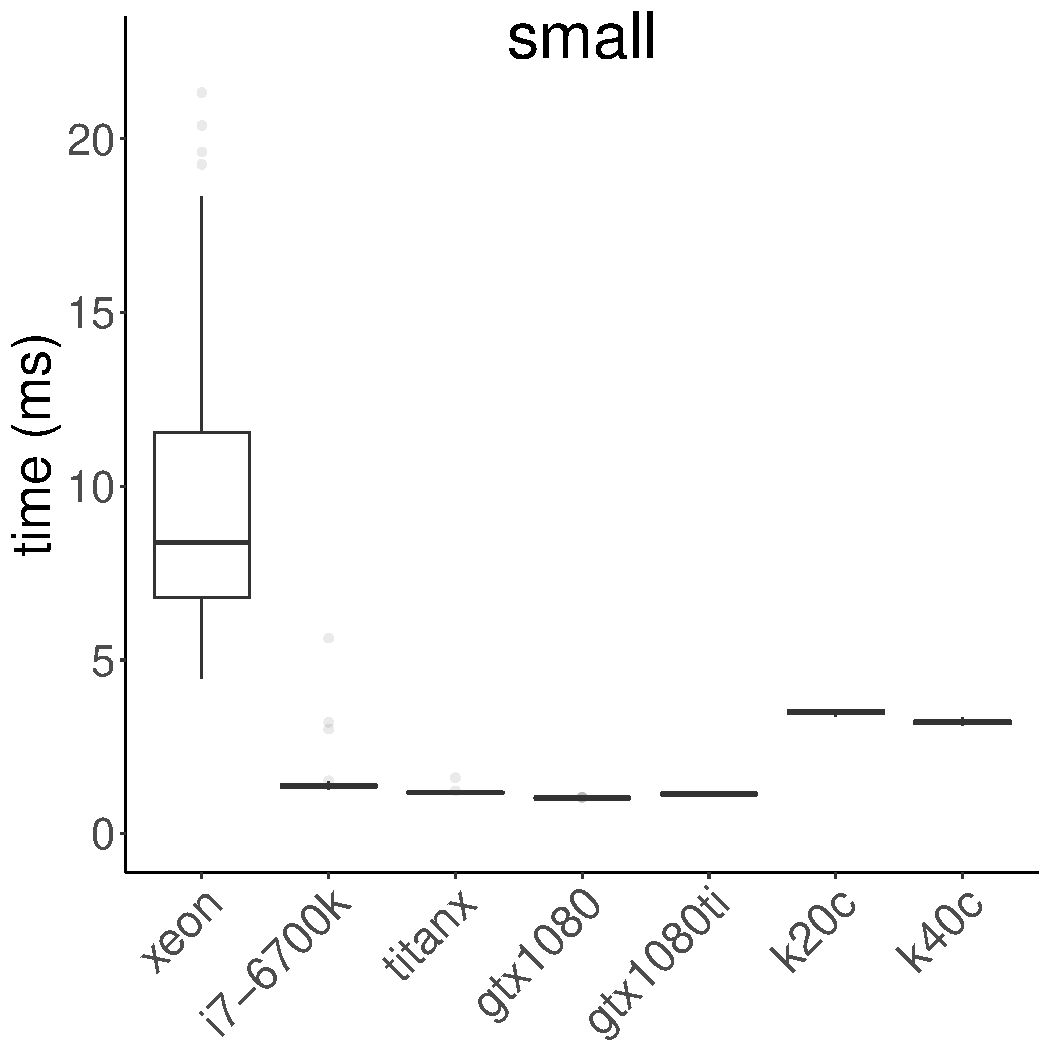
\includegraphics[width=\plotwidth]{figures/time-results/generate_kmeans_no_knl_small_boxplot-1}
		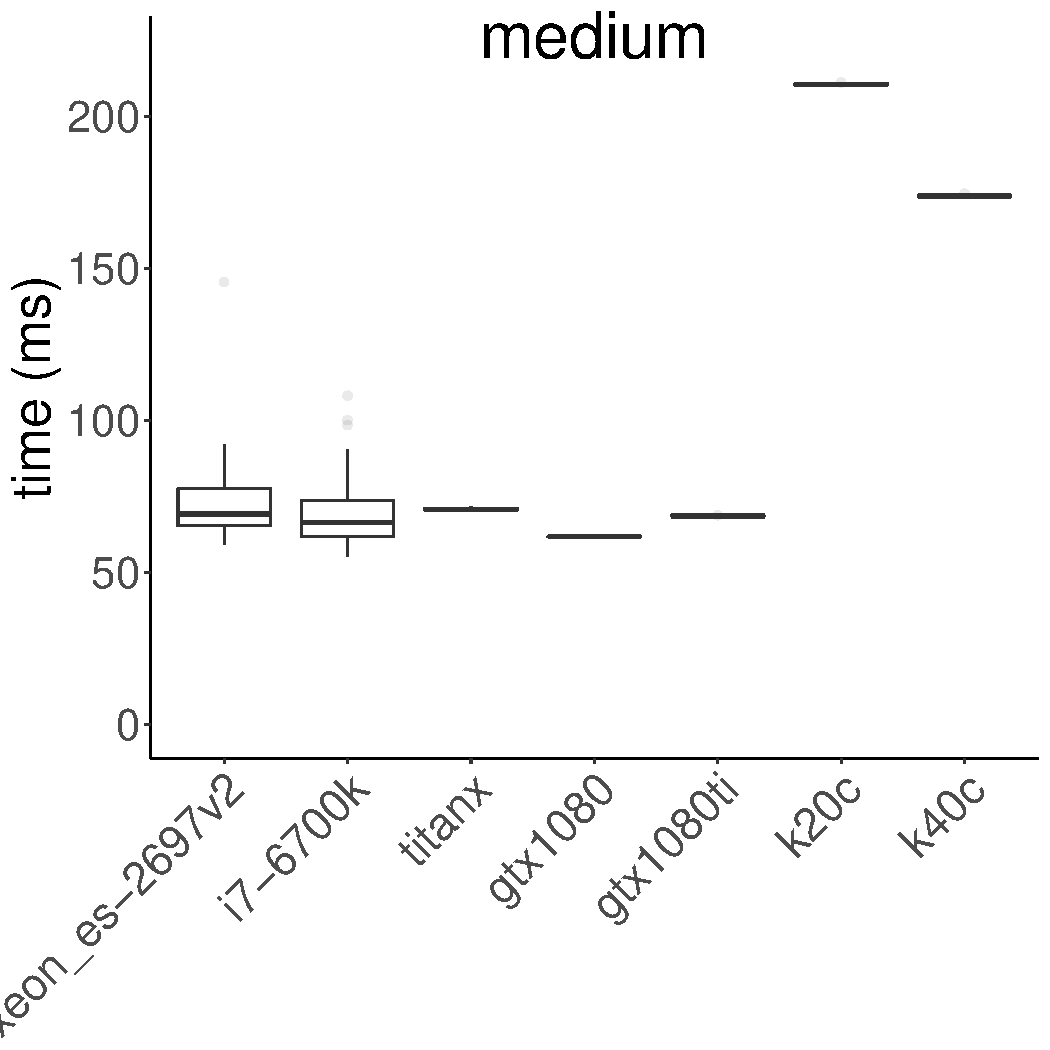
\includegraphics[width=\plotwidth]{figures/time-results/generate_kmeans_no_knl_medium_boxplot-1}
		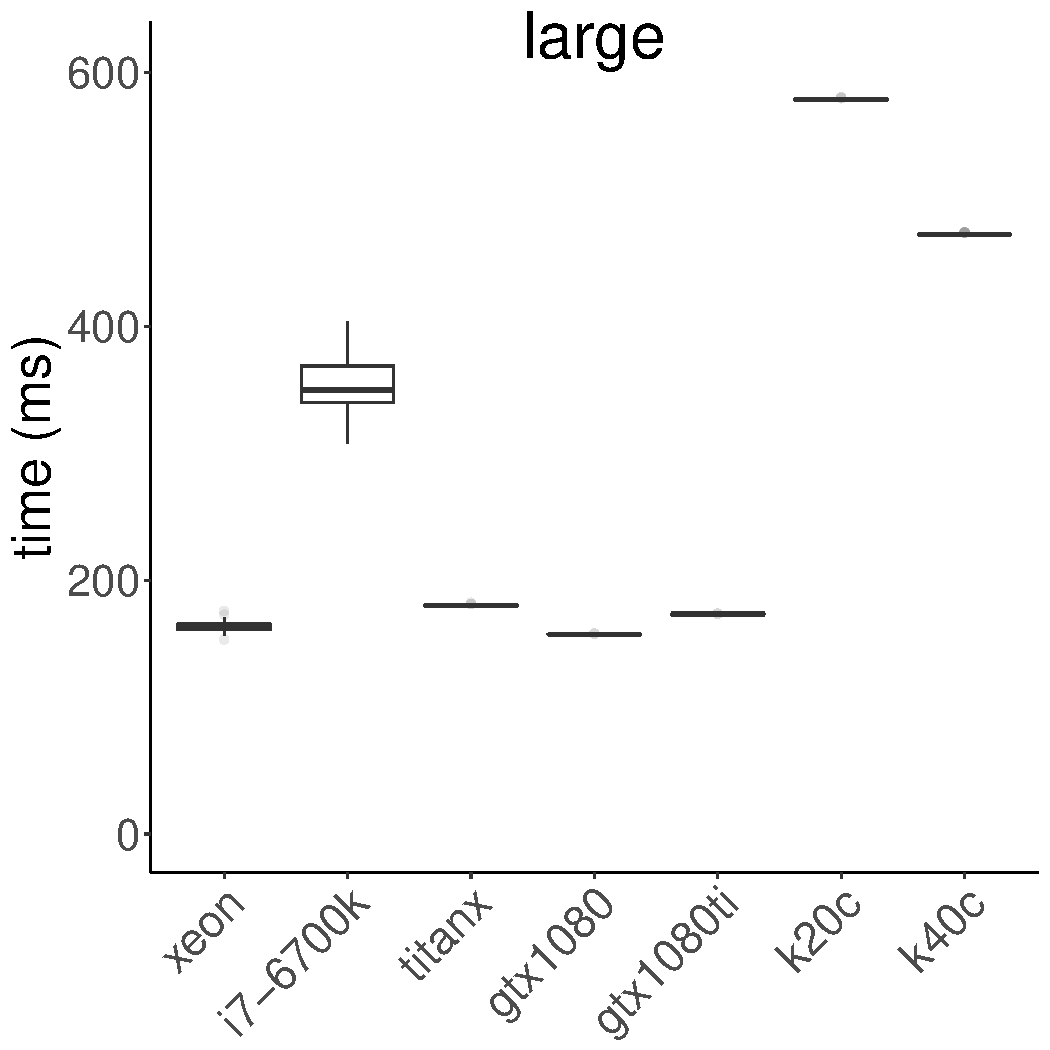
\includegraphics[width=\plotwidth]{figures/time-results/generate_kmeans_no_knl_large_boxplot-1}
	\end{subfigure}

	\begin{subfigure}{0.09\textwidth}\subcaption[l]{\bf lud} \label{fig:time-lud} \vspace{5mm}\end{subfigure}
	\begin{subfigure}{0.9\textwidth}
		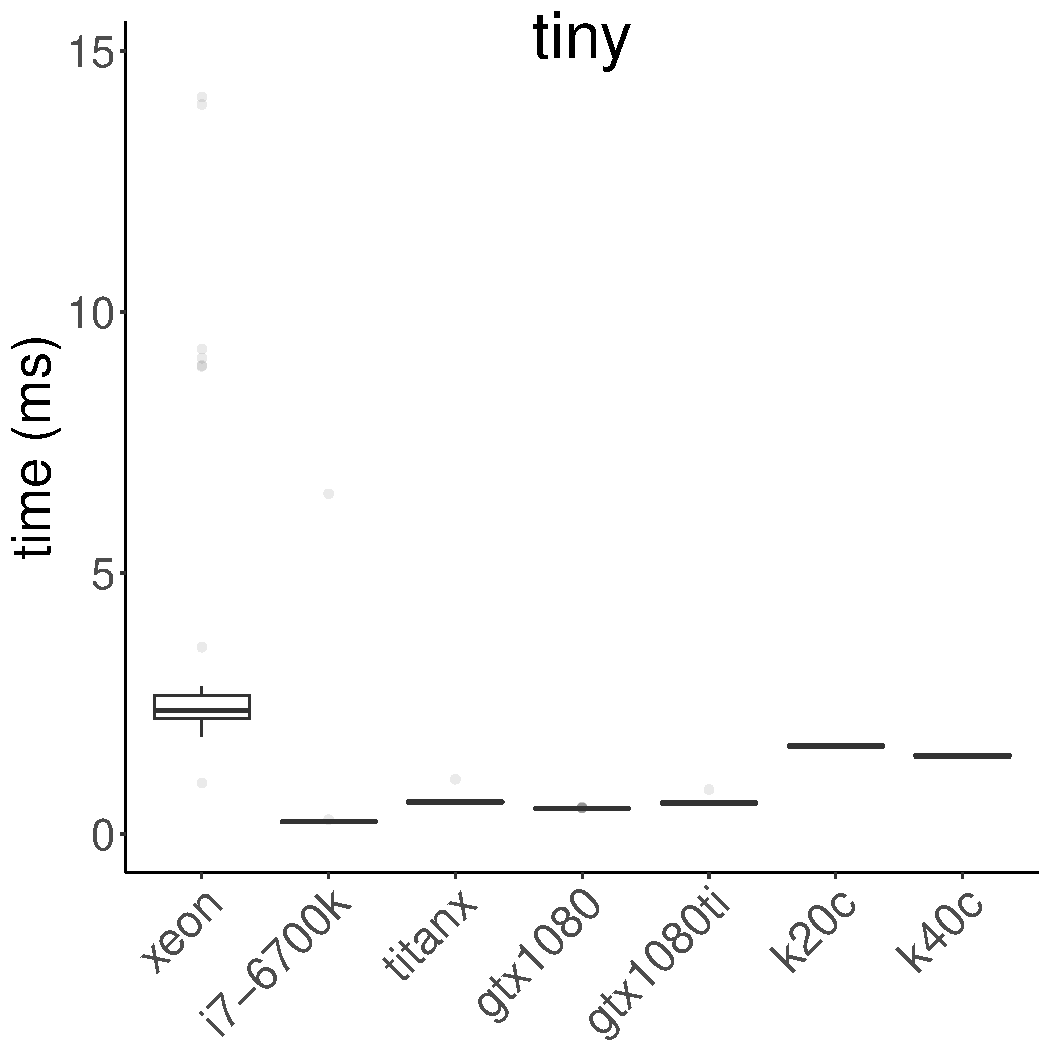
\includegraphics[width=\plotwidth]{figures/time-results/generate_lud_tiny_boxplot-1}
		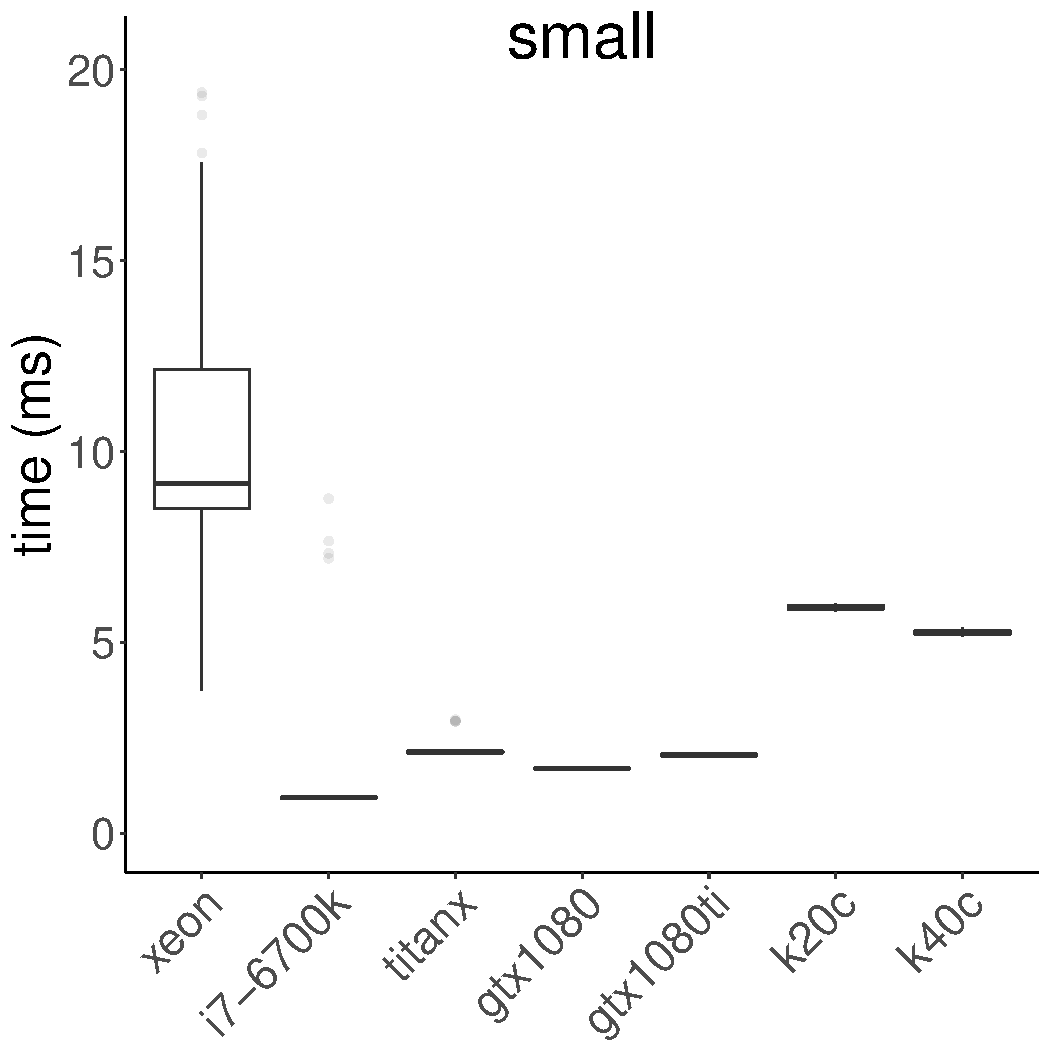
\includegraphics[width=\plotwidth]{figures/time-results/generate_lud_small_boxplot-1}
		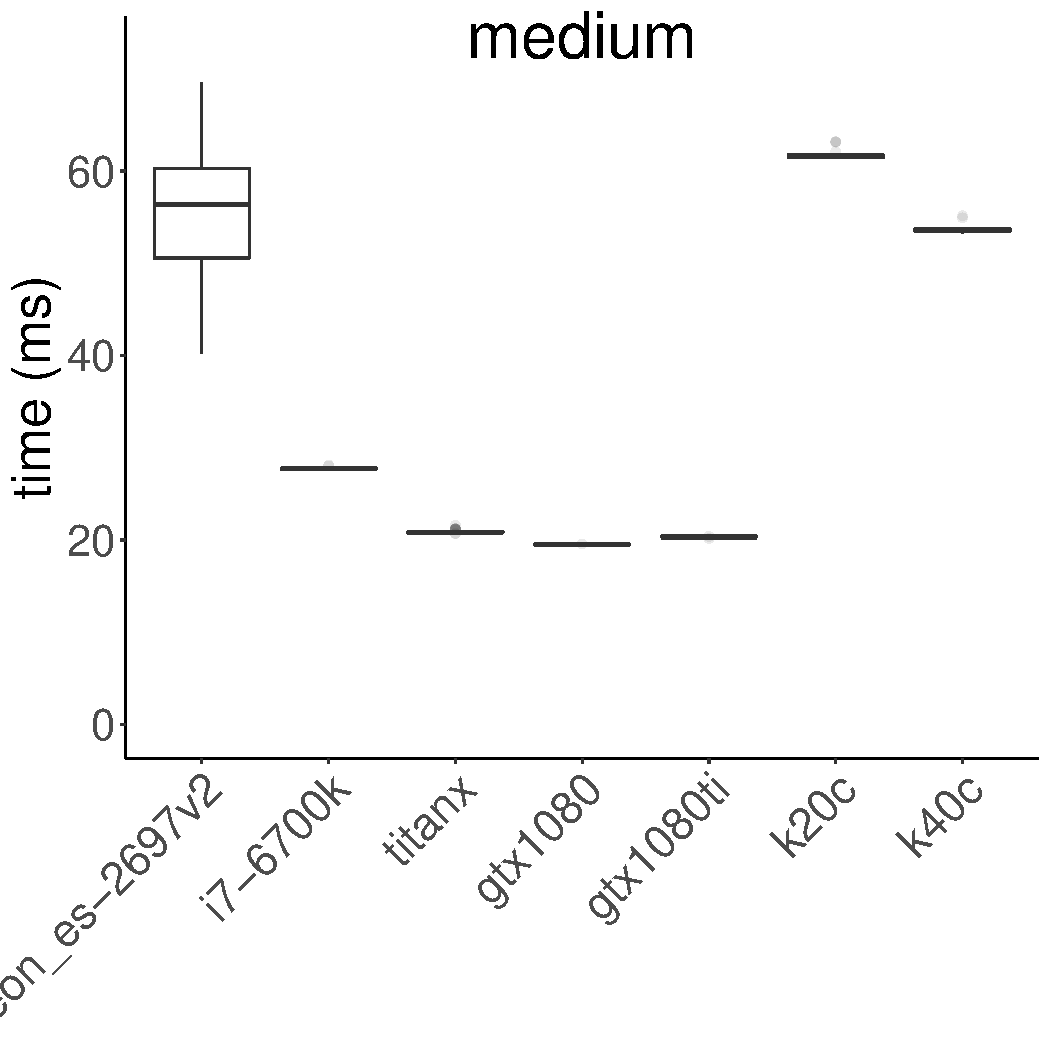
\includegraphics[width=\plotwidth]{figures/time-results/generate_lud_medium_boxplot-1}
		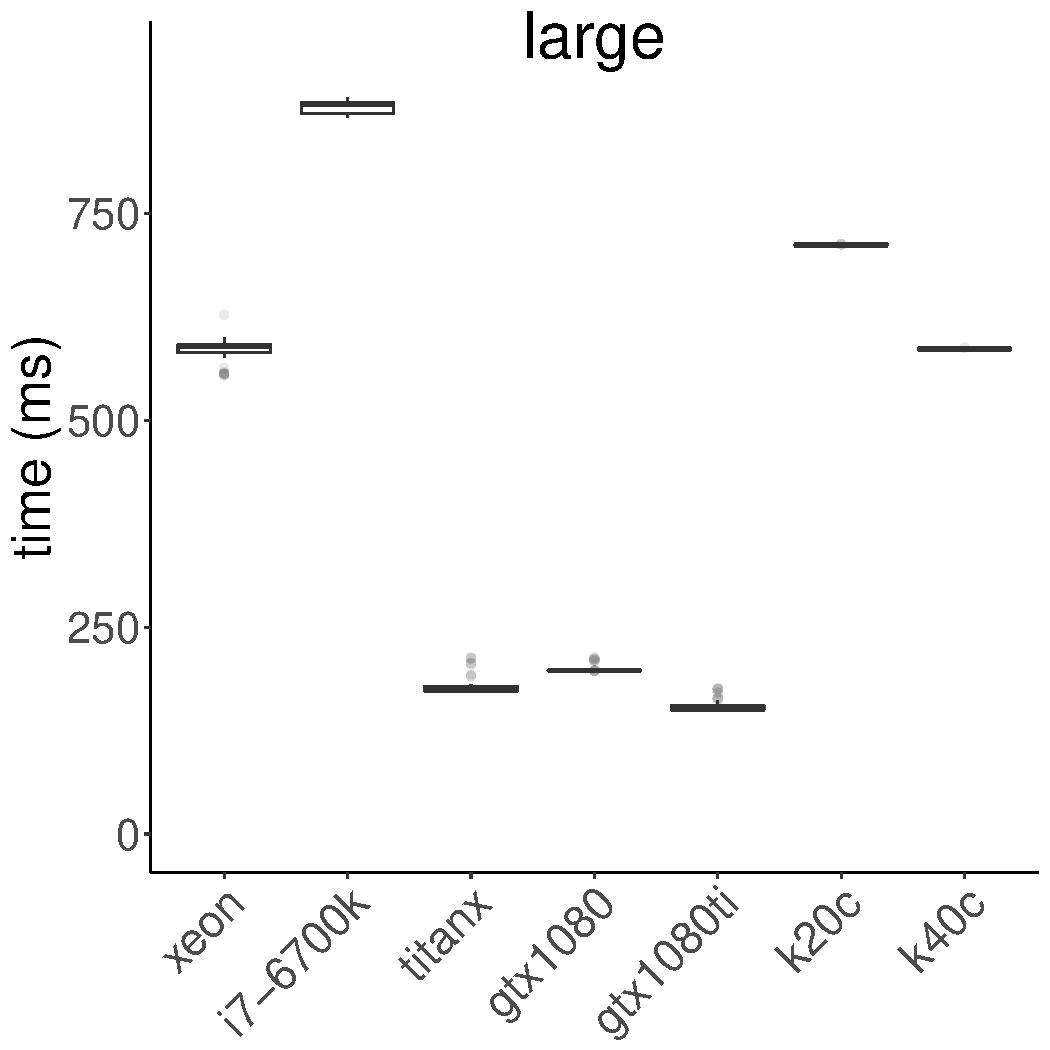
\includegraphics[width=\plotwidth]{figures/time-results/generate_lud_large_boxplot-1}
	\end{subfigure}

	\begin{subfigure}{0.09\textwidth}\subcaption[l]{\bf csr} \label{fig:time-csr} \vspace{5mm}\end{subfigure}
	\begin{subfigure}{0.9\textwidth}
		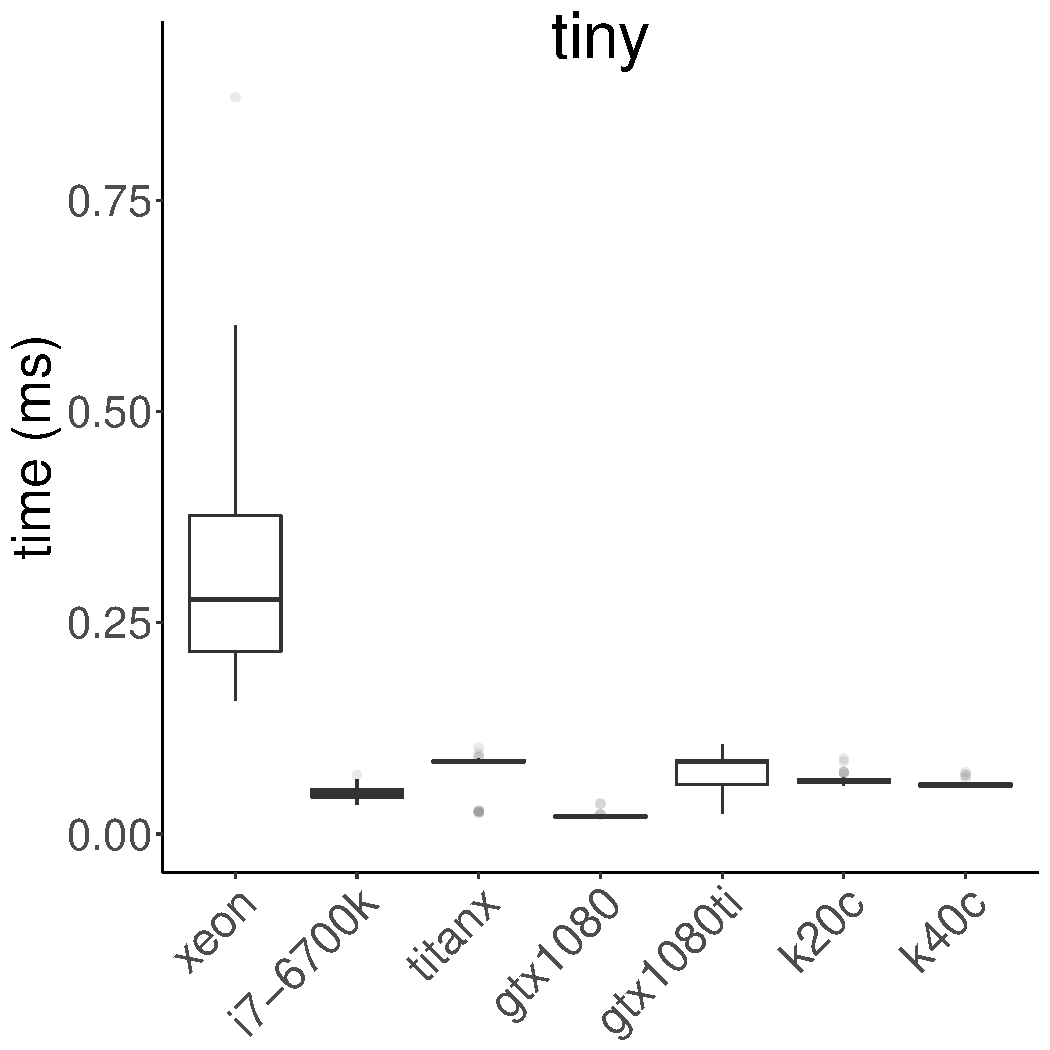
\includegraphics[width=\plotwidth]{figures/time-results/generate_csr_tiny_boxplot-1}
		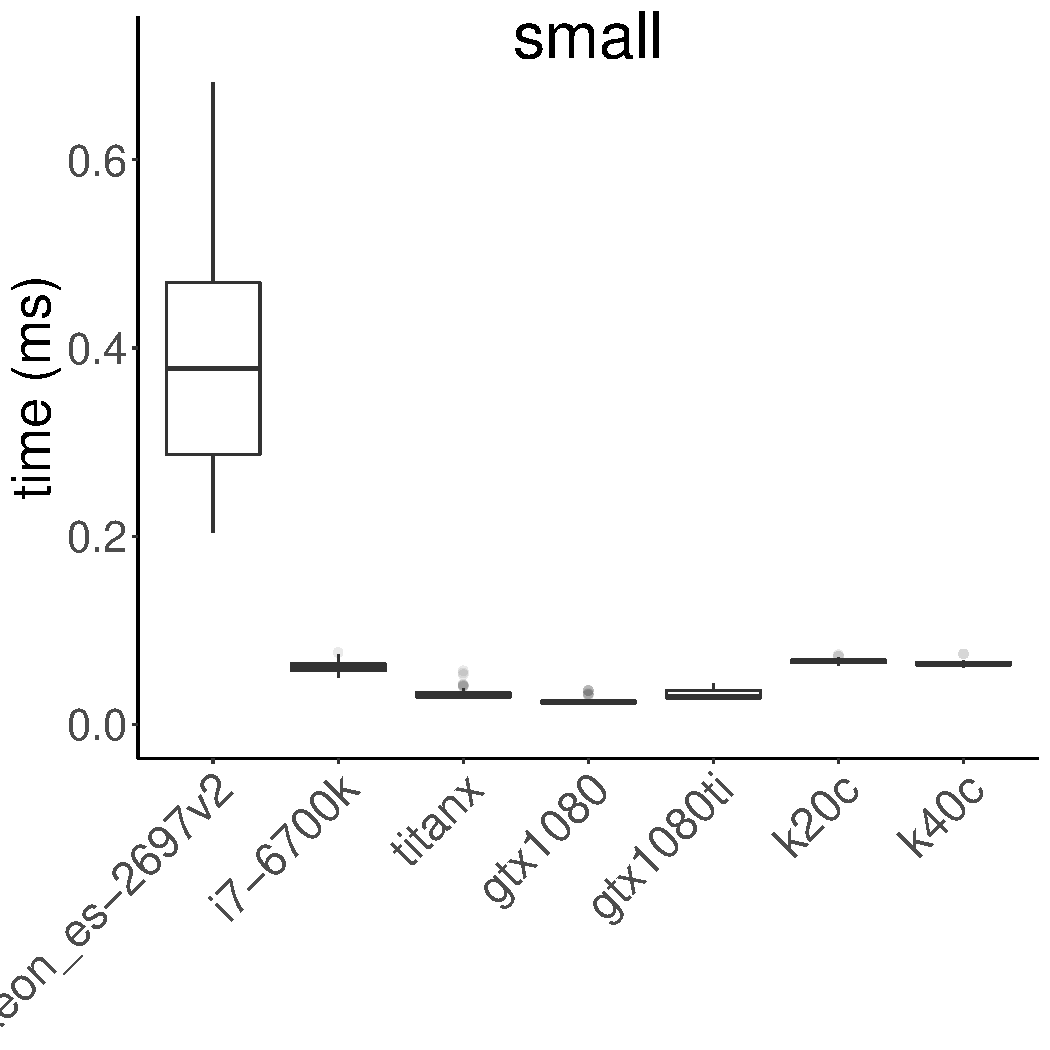
\includegraphics[width=\plotwidth]{figures/time-results/generate_csr_small_boxplot-1}
		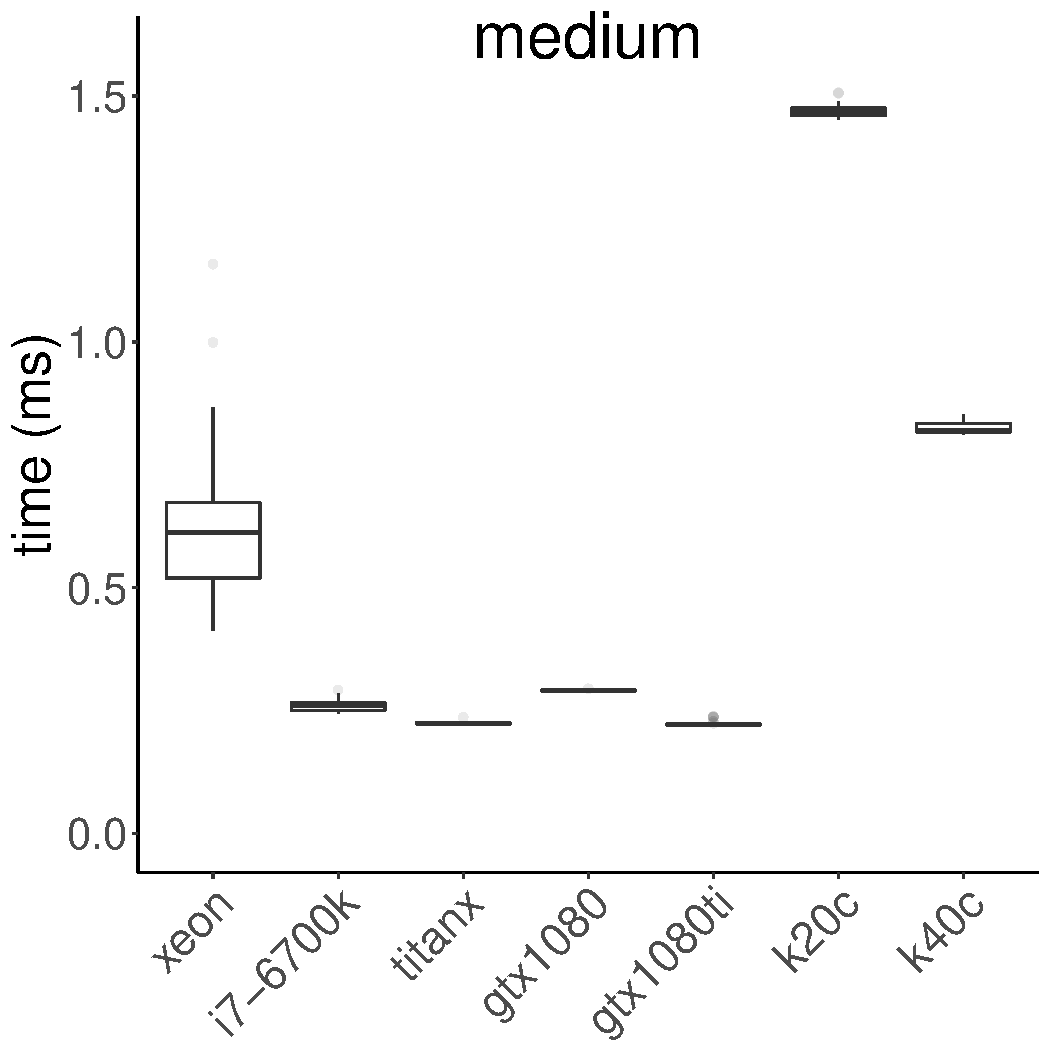
\includegraphics[width=\plotwidth]{figures/time-results/generate_csr_medium_boxplot-1}
		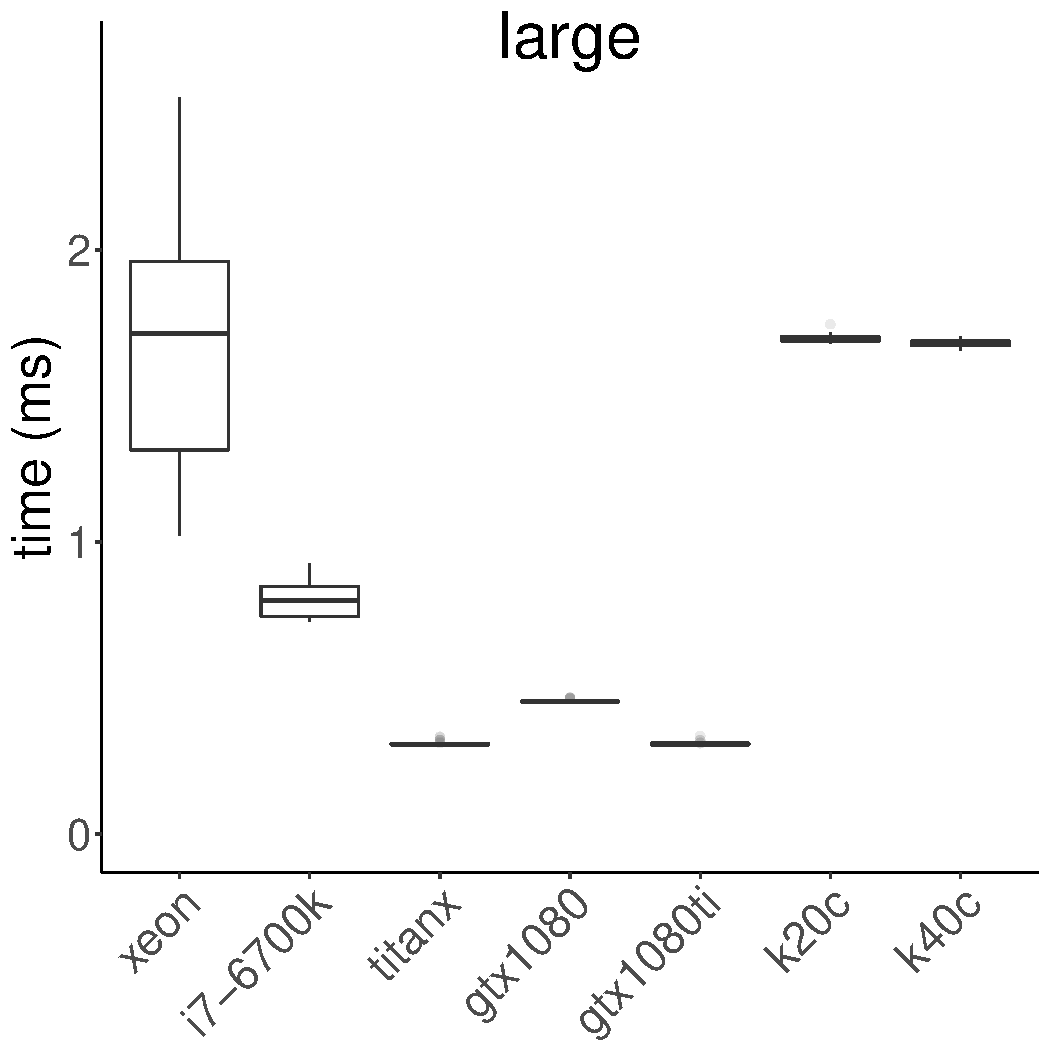
\includegraphics[width=\plotwidth]{figures/time-results/generate_csr_large_boxplot-1}
	\end{subfigure}
	
	\begin{subfigure}{0.09\textwidth}\subcaption[l]{\bf dwt} \label{fig:time-dwt} \vspace{5mm}\end{subfigure}
	\begin{subfigure}{0.9\textwidth}
		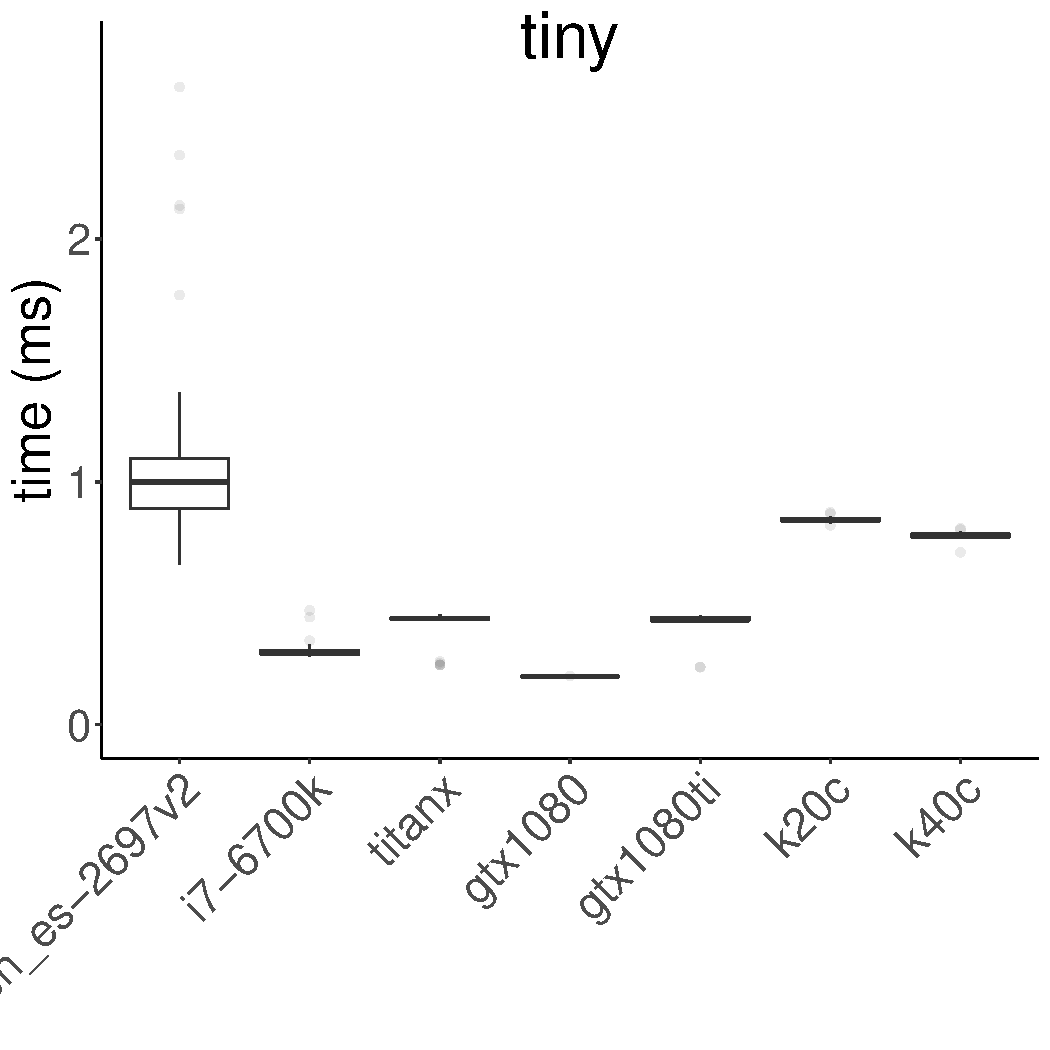
\includegraphics[width=\plotwidth]{figures/time-results/generate_dwt_tiny_boxplot-1}
		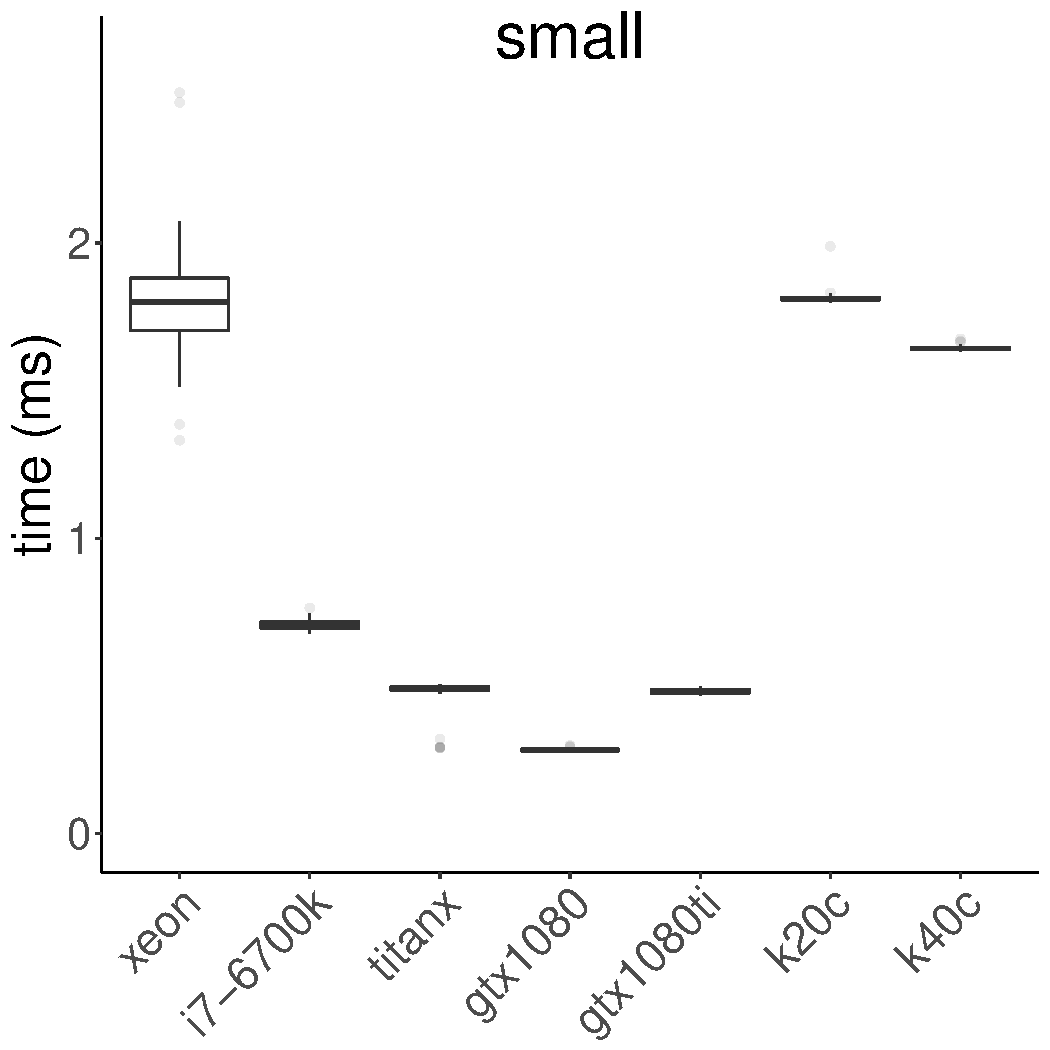
\includegraphics[width=\plotwidth]{figures/time-results/generate_dwt_small_boxplot-1}
		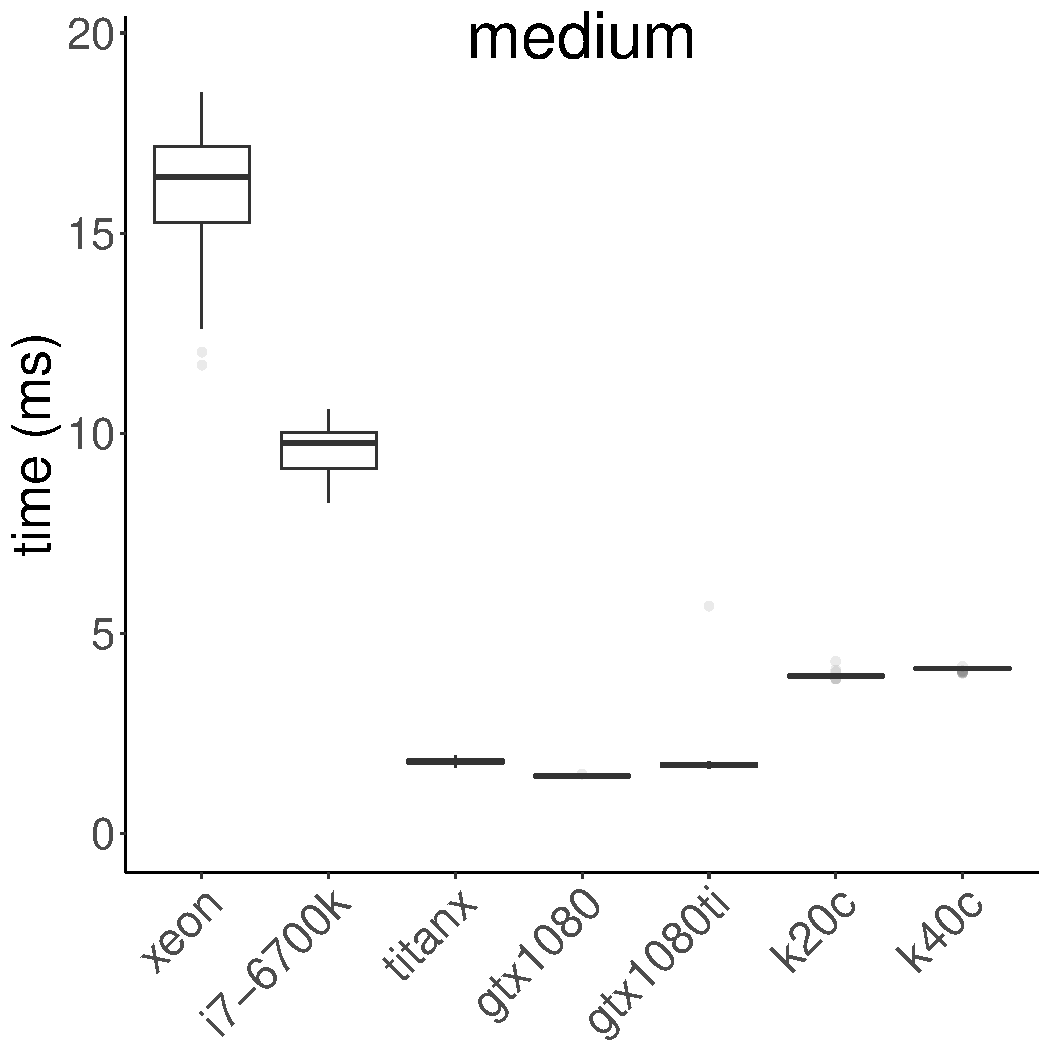
\includegraphics[width=\plotwidth]{figures/time-results/generate_dwt_medium_boxplot-1}
		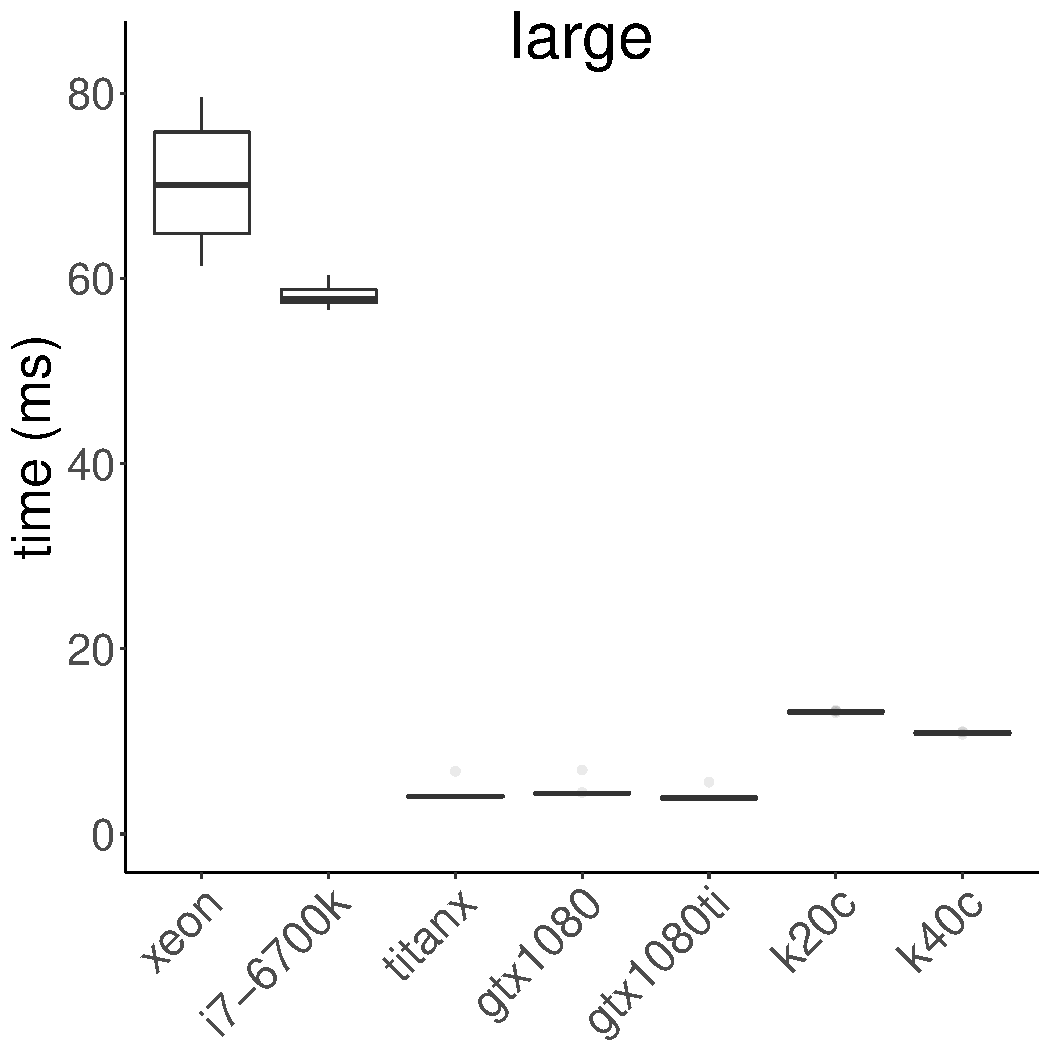
\includegraphics[width=\plotwidth]{figures/time-results/generate_dwt_large_boxplot-1}
	\end{subfigure}

	\begin{subfigure}{0.09\textwidth}\subcaption[l]{\bf fft} \label{fig:time-fft} \vspace{5mm}\end{subfigure}
	\begin{subfigure}{0.9\textwidth}
		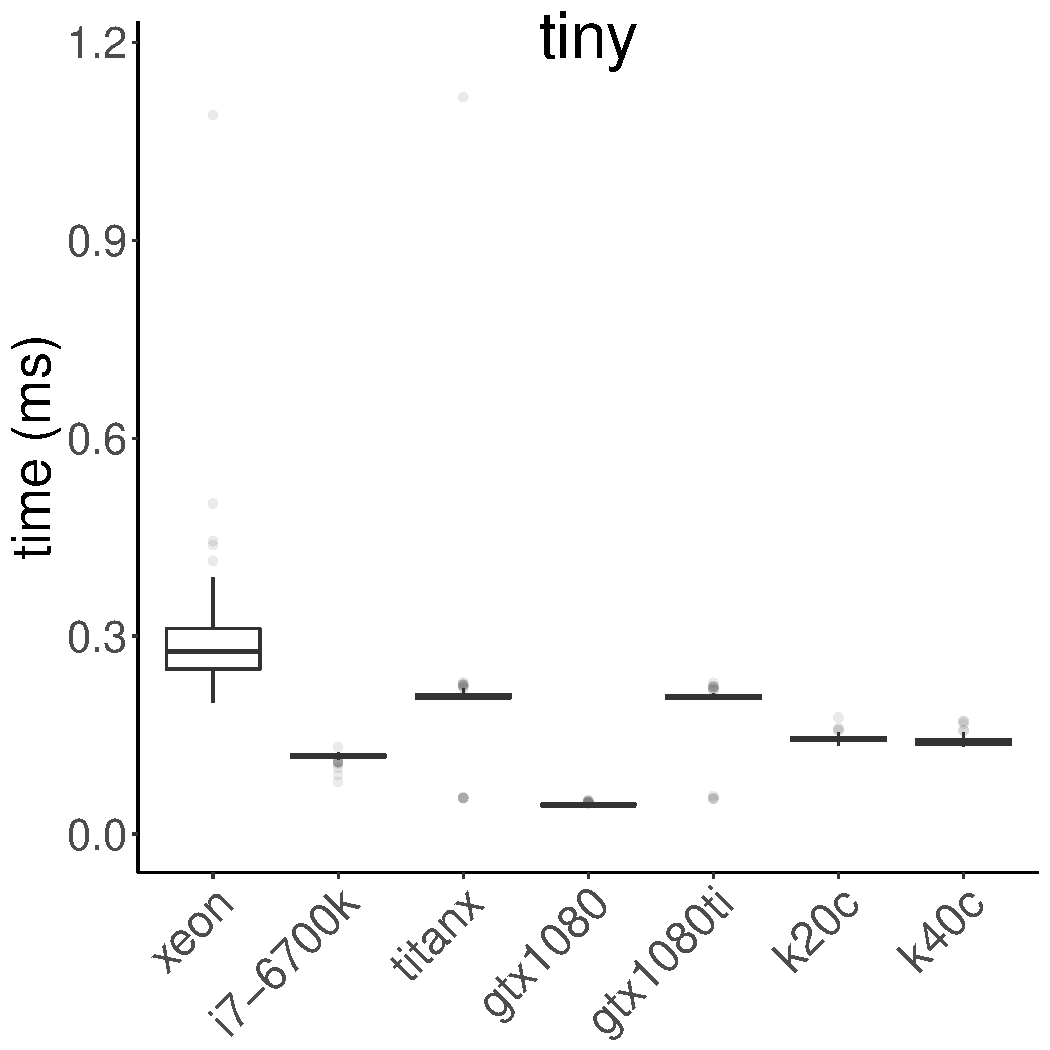
\includegraphics[width=\plotwidth]{figures/time-results/generate_fft_tiny_boxplot-1}
		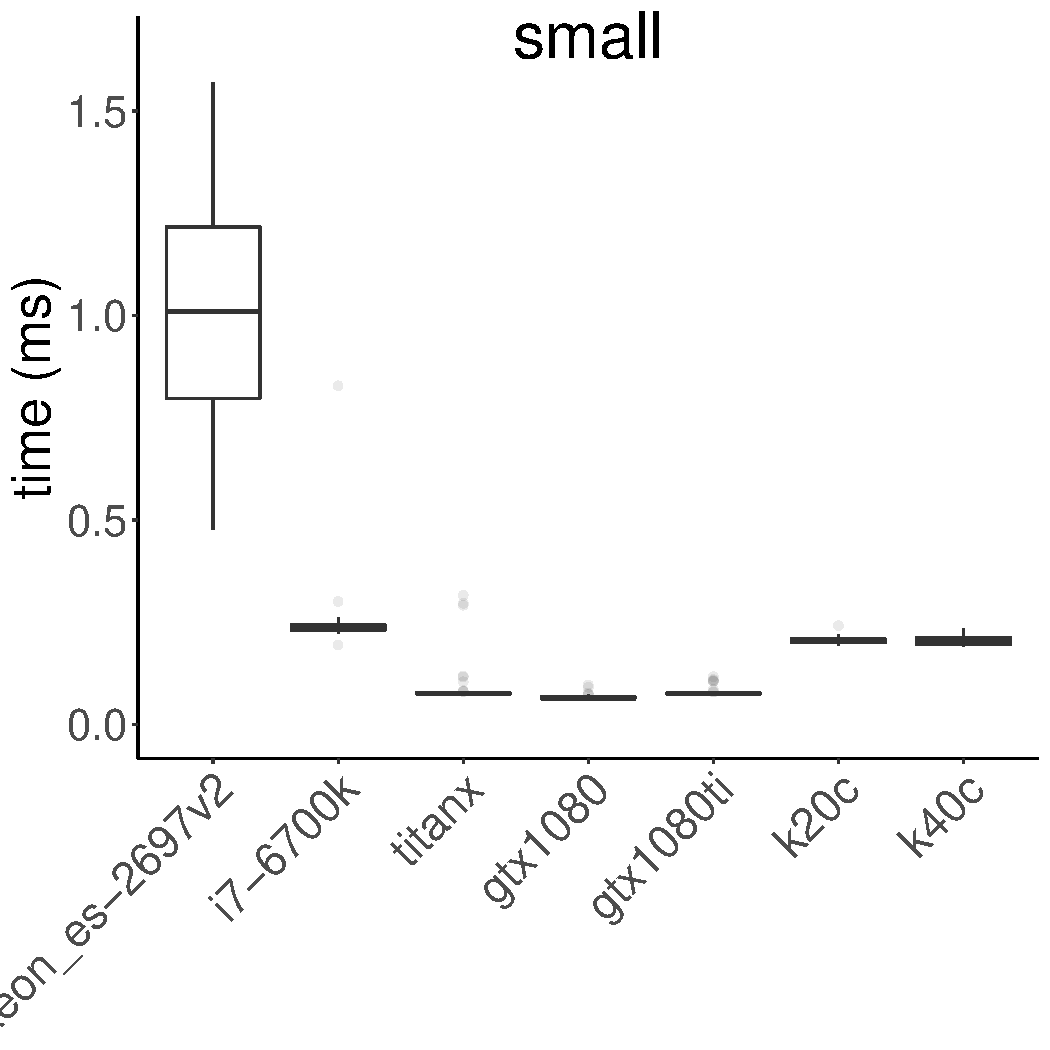
\includegraphics[width=\plotwidth]{figures/time-results/generate_fft_small_boxplot-1}
		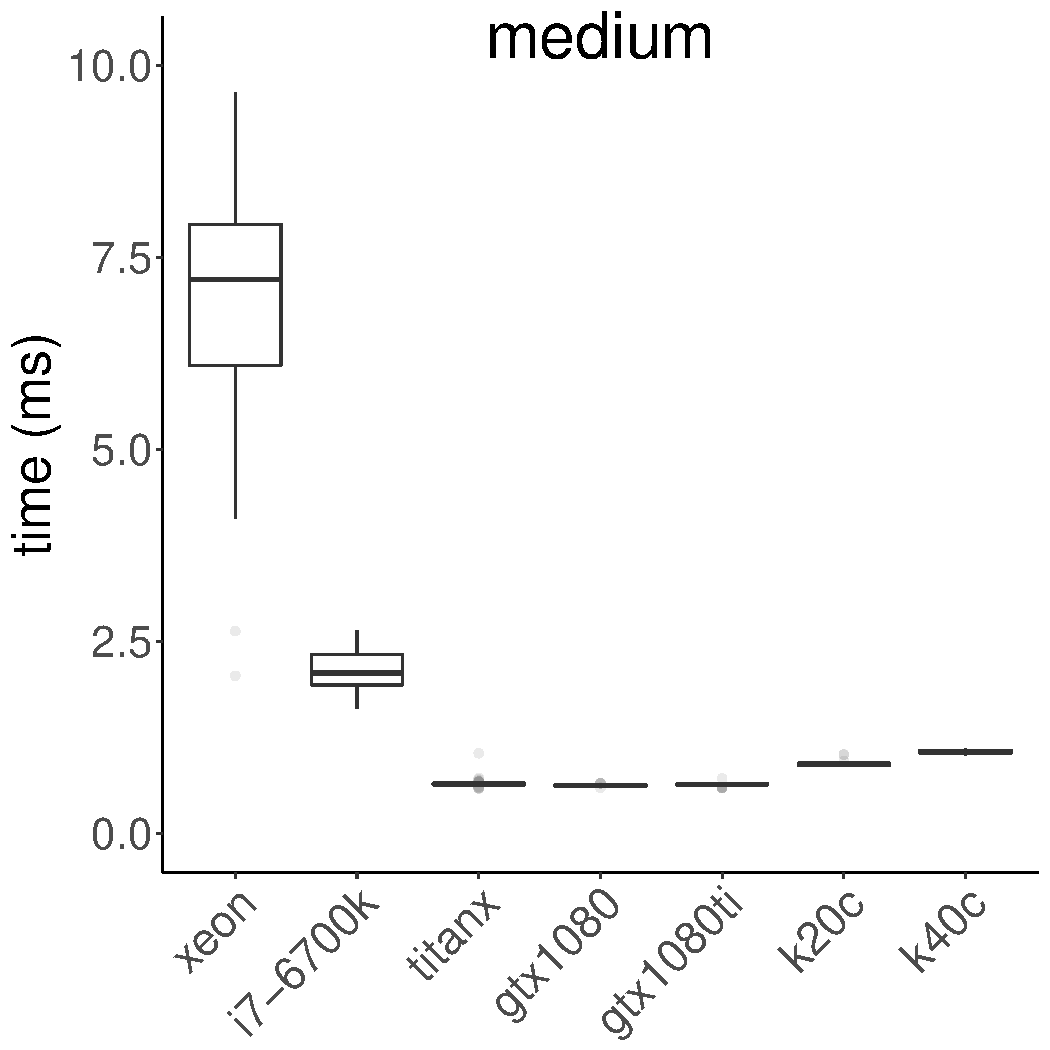
\includegraphics[width=\plotwidth]{figures/time-results/generate_fft_medium_boxplot-1}
		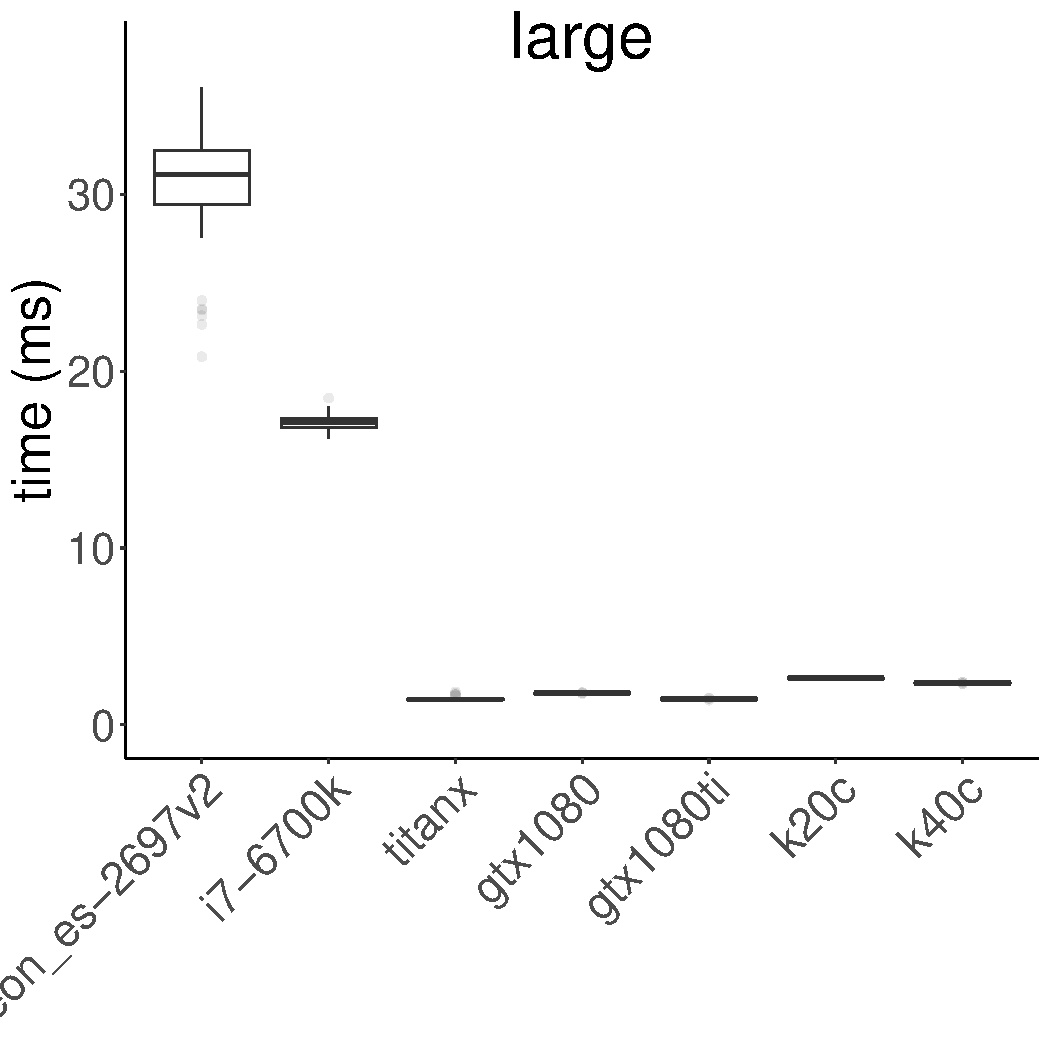
\includegraphics[width=\plotwidth]{figures/time-results/generate_fft_large_boxplot-1}
	\end{subfigure}
    \caption{Benchmark kernel execution times on different hardware platforms}\label{fig:time}
\end{figure*}

\begin{figure*}[t]
	\begin{subfigure}{0.09\textwidth}\subcaption[l]{\bf gem} \label{fig:time-gem} \vspace{5mm}\end{subfigure}
	\begin{subfigure}{0.9\textwidth}
		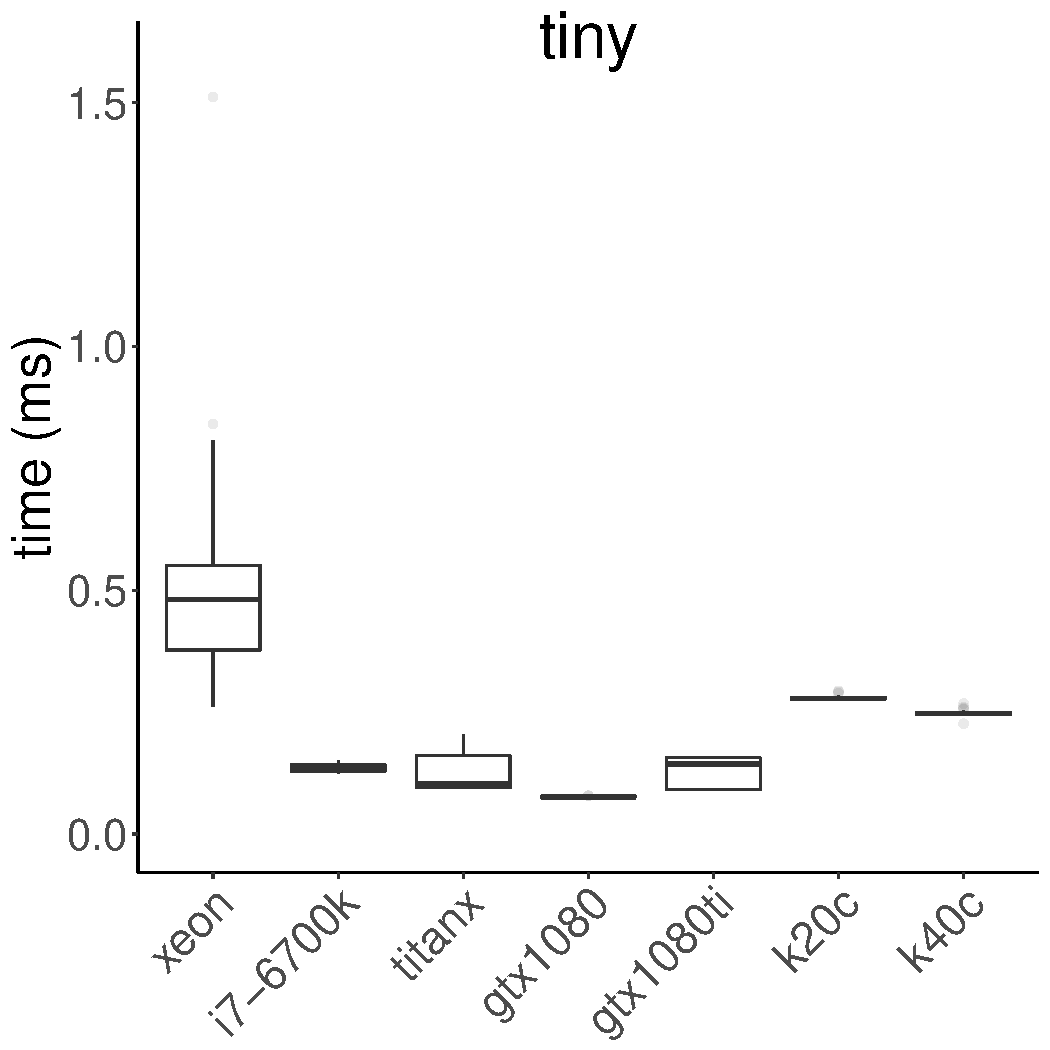
\includegraphics[width=\plotwidth]{figures/time-results/generate_gem_tiny_boxplot-1}
		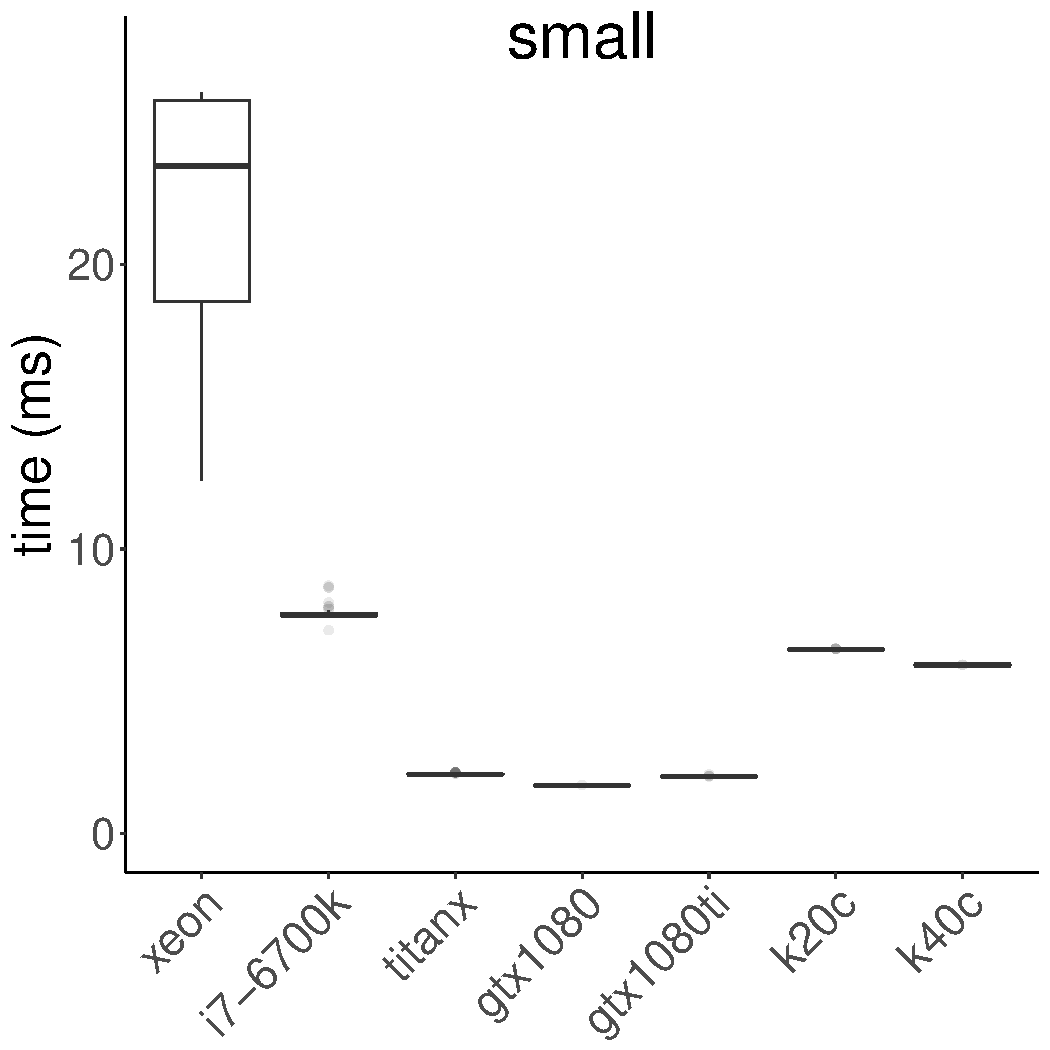
\includegraphics[width=\plotwidth]{figures/time-results/generate_gem_small_boxplot-1}
		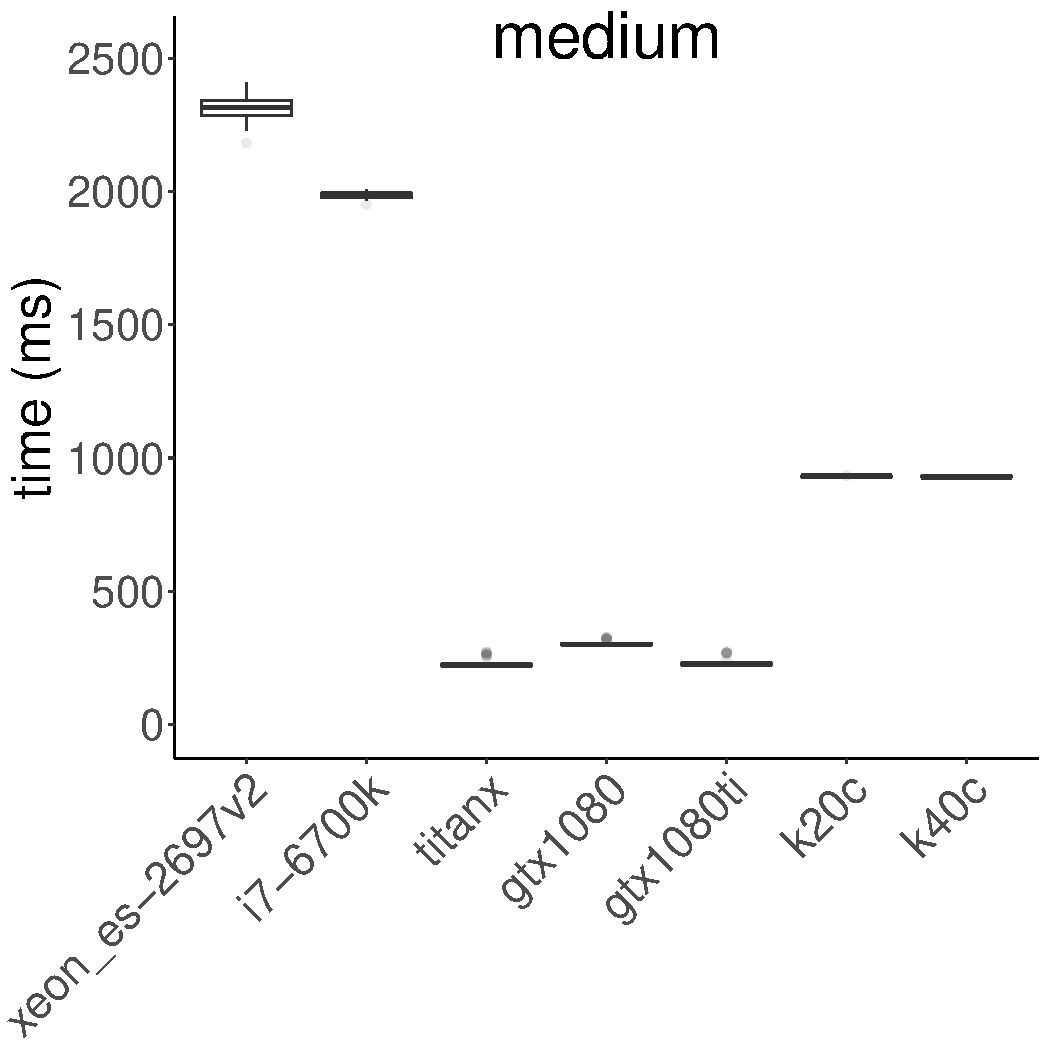
\includegraphics[width=\plotwidth]{figures/time-results/generate_gem_medium_boxplot-1}
		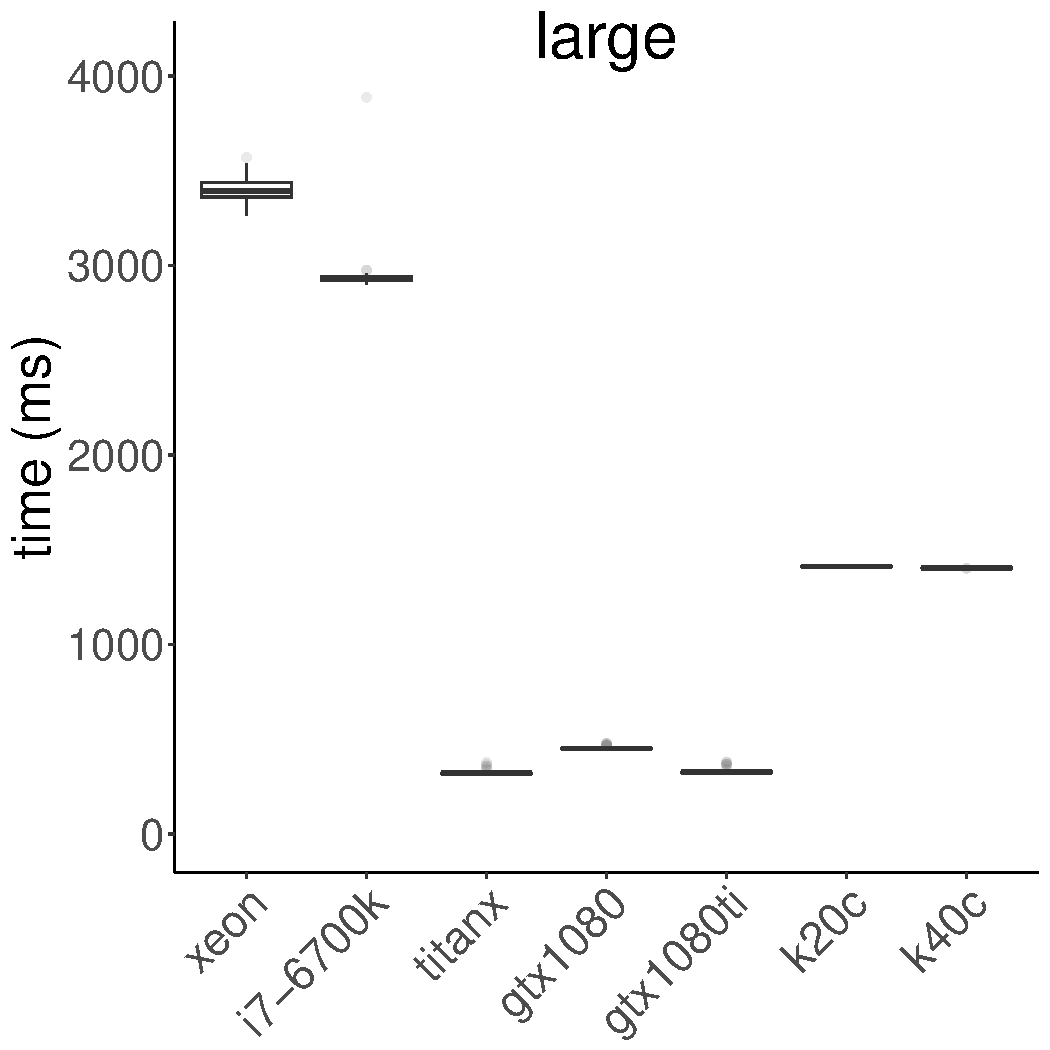
\includegraphics[width=\plotwidth]{figures/time-results/generate_gem_large_boxplot-1}
		\end{subfigure}

	\begin{subfigure}{0.09\textwidth}\subcaption[l]{\bf srad} \label{fig:time-srad} \vspace{5mm}\end{subfigure}
	\begin{subfigure}{0.9\textwidth}
		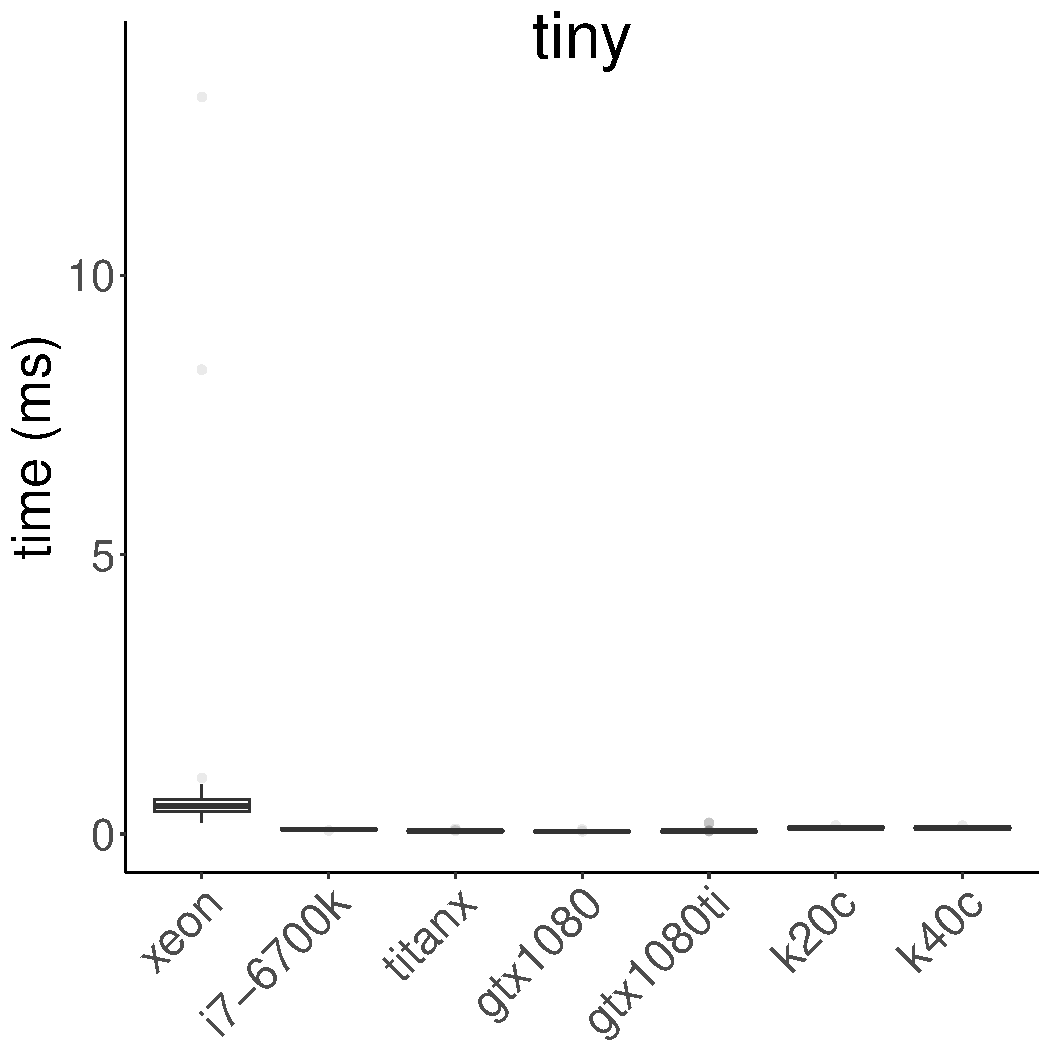
\includegraphics[width=\plotwidth]{figures/time-results/generate_srad_tiny_boxplot-1}
		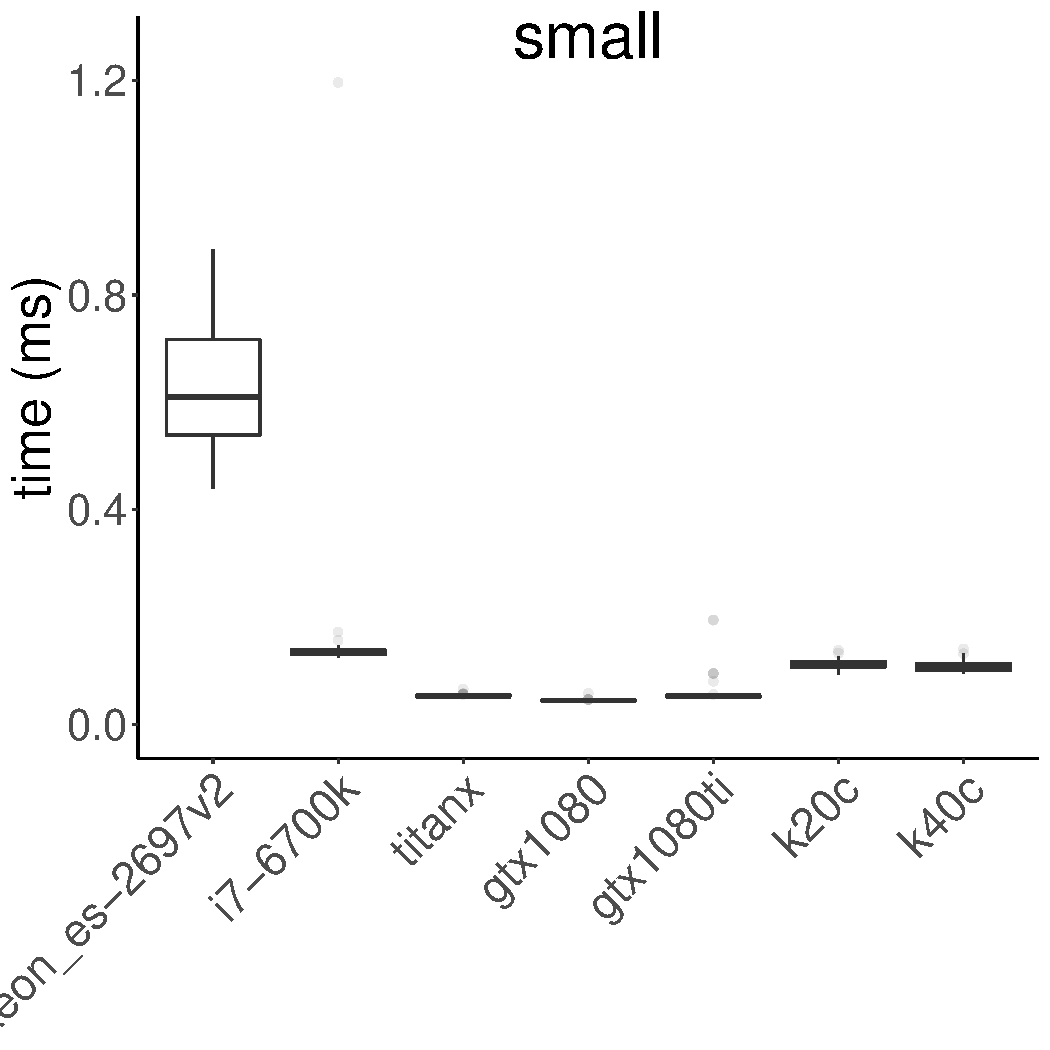
\includegraphics[width=\plotwidth]{figures/time-results/generate_srad_small_boxplot-1}
		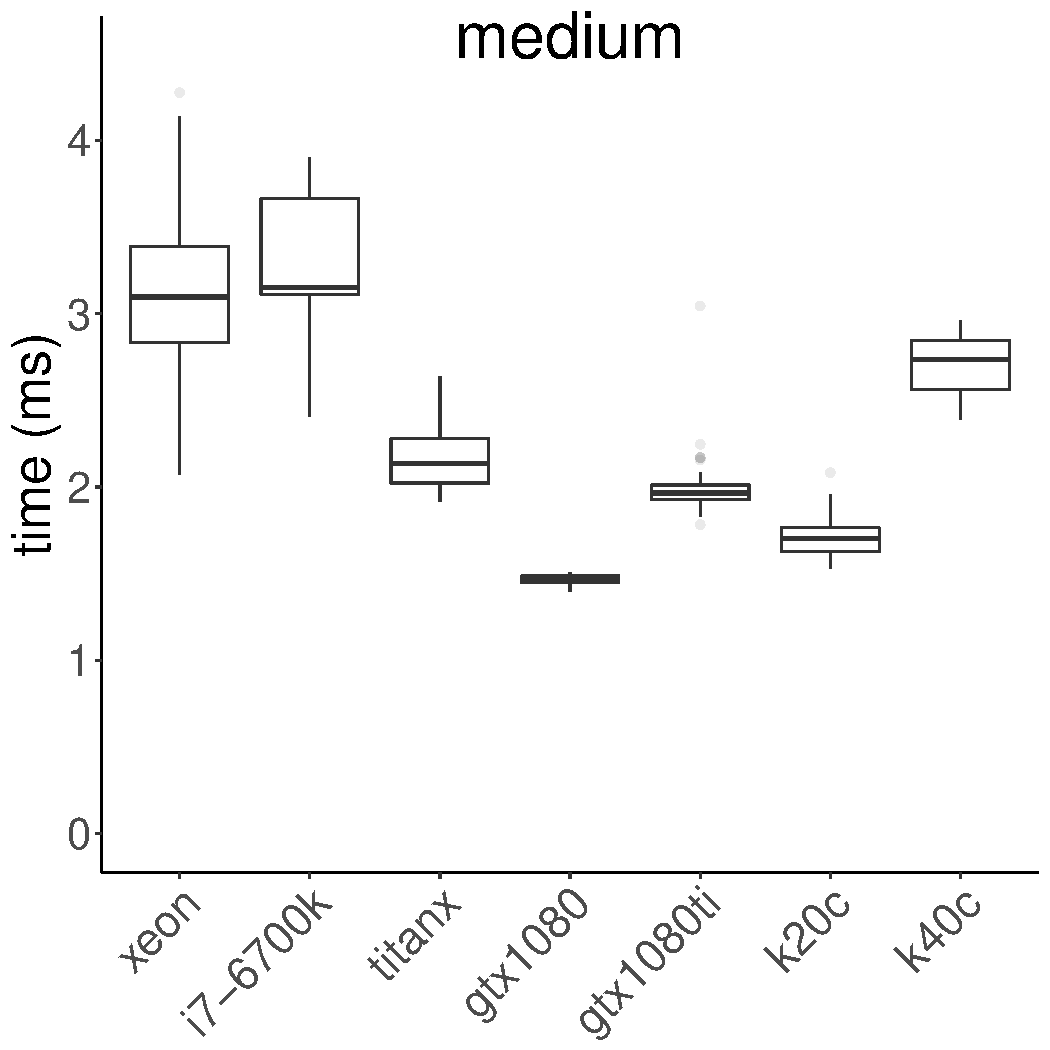
\includegraphics[width=\plotwidth]{figures/time-results/generate_srad_medium_boxplot-1}
		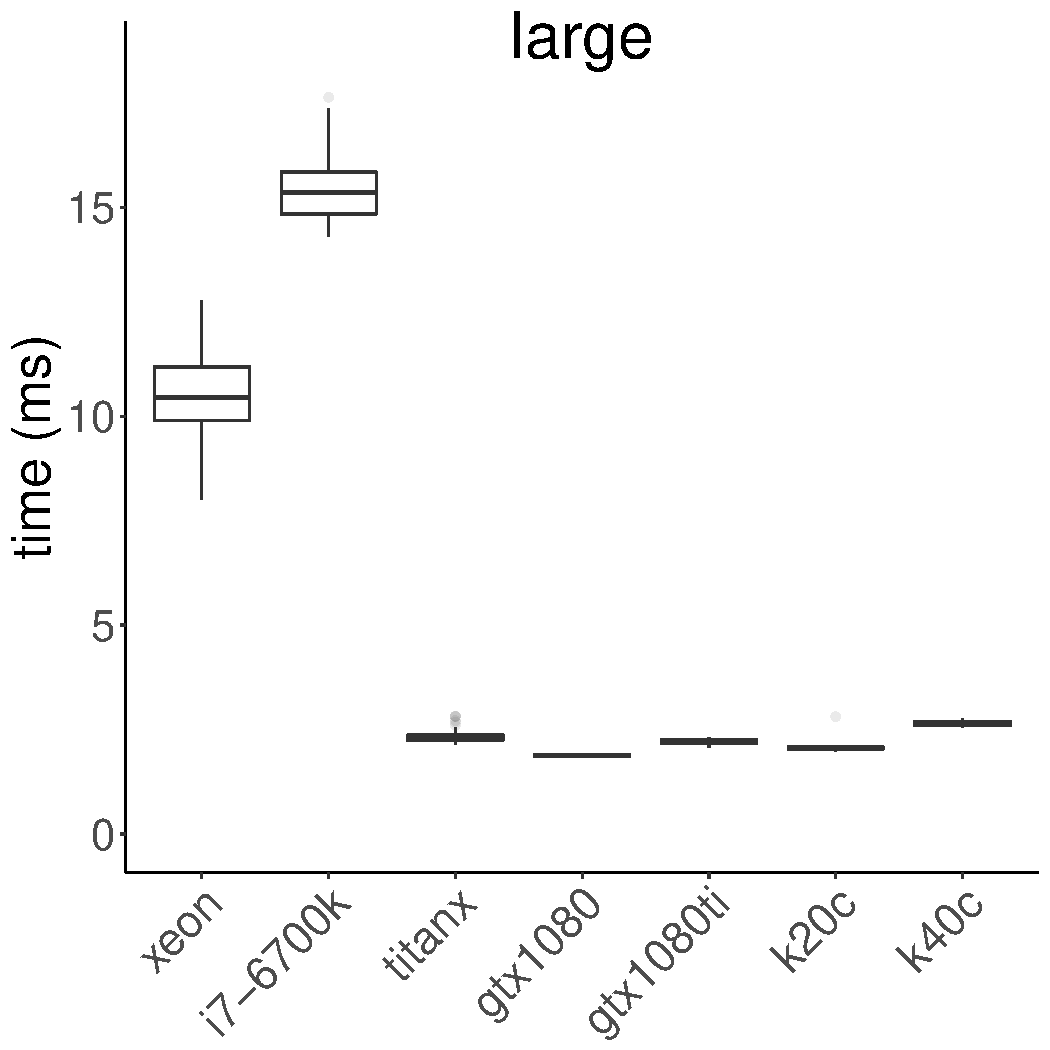
\includegraphics[width=\plotwidth]{figures/time-results/generate_srad_large_boxplot-1}
	\end{subfigure}
    \caption{Benchmark kernel execution times on different hardware platforms (continued)}\label{fig:time2}
\end{figure*}

For most benchmarks, the variance in execution times is much greater on the CPU platforms than on GPUs.
\todo[inline]{Why? Possibly due to cycles run at lower clock speeds? Does clock throttling affect GPU as well?}
While execution time increases with problem size for all benchmarks and platforms, the modern GPUs (Titan X, GTX1080 and GTX1080i) performed relatively better for large problem sizes, possibly due to their greater second-level cache size compared to the other platforms.
A notable exception is {\tt k-means} for which CPU execution times were comparable to GPU, which reflects the relatively low ratio of floating point to memory operations in the benchmark.

\todo{runtime results -- why they are what they are and how the use of OpenCL itself helps/hinders performance}
\todo{Are there any benchmarks where increasing the problem sizes makes results worse for the GPU?}
\todo{How does changing problem sizes affect benchmark performance across a range of platforms (selected accordingly to cache size)?}
\todo{Comment on the similarities within a dwarf and the differences between them.}

\end{document}
